% =====================================================================
%  Chapter 6 -- Assessment of AI Training Datasets Trustworthiness
%
%  Revised 2026-09 following F. Kargl's review of 2026-06-24 (73 comments,
%  see reviews/ch06-fk-review-2026-06-24.md). Main changes:
%   * scope / contributions / roadmap added to the introduction;
%   * Sec. 6.2 re-grounded in dataset examples instead of re-introducing Ch. 2;
%   * Phase I = structure (tree + trust-source catalogue), Phase II =
%     quantification (metric -> evidence -> opinion, hyperparameters);
%   * every application states its purpose / research question, introduces
%     its dataset, and closes with "what this example showed";
%   * terminology unified: trust source (not metric), belief/disbelief (b,d,u).
%
%  Labels follow chap6:* / sec:* / fig:* / tab:* / eq:* conventions.
% =====================================================================

\chapter{Assessment of AI Training Datasets Trustworthiness}
\label{chap:dataset-trust}
\acresetall
The previous chapter presented the overall architecture of \ac{PaTAS}, highlighting its two main components: (i) the Trust Assessment Module, which assesses the trustworthiness of the training dataset and of the input of the \ac{NN}, and (ii) the Trust Propagation Module, which propagates trust through the model, from the training data to the learned parameters and from the input to the output via these parameters. This chapter focuses on the first component, the trust assessment module. The underlying ideas were initially explored in the paper presented at the BIAS Workshop at ECML PKDD~\cite{10.1007/978-3-032-19096-3_17} and further developed in the paper on labeling accuracy presented at the TRUST-AI Workshop of ECAI~\cite{trust-aidatatrust}. In this dissertation, these contributions are unified and extended into a single framework for assessing the trustworthiness of training datasets.

% --------------------------------------------------------------
\section{Introduction}
\label{sec:dataset-trust:intro}

The chapter is organized around three observations. First, \emph{the trustworthiness of a training dataset is not a scalar.} Different trustworthiness properties such as fairness, correctness, representativeness, privacy compliance, and robustness to leakage require different types of evidence, different evaluation granularities, and different aggregation rules. Collapsing them into a single quality score, or applying the same metric, the same threshold, and the same aggregation rule across all of them, hides exactly the information that should drive downstream decisions: which property is at risk, at which stage of the lifecycle.

Second, \emph{properties live at different levels of the data}. Some properties are only meaningful at the \textbf{dataset level} (e.g., class balance, coverage). Others are intrinsically \textbf{per-entry} (e.g., label correctness) or \textbf{per-feature} (e.g., the reliability of an individual sensor channel).

Third, \emph{evidence about trustworthiness is rarely complete}. Training datasets are typically constructed through multi-stage lifecycles in which documentation, metadata, and direct observations are partial, sometimes contradictory, and often unavailable for historical pipelines. The framework must therefore distinguish \emph{low support} from \emph{no support}, which is exactly what \aclu{SL} offers and what scalar quality scores cannot.

\paragraph{Scope.}
The object of this chapter is the \emph{training dataset} $\dataset$ of a \ac{NN}: the collection of entries (rows, images, records) and their labels that the model is trained on. The framework produces trust opinions about $\dataset$, or about parts of it, with respect to a stated property. Inputs presented to the model at inference time are \emph{not} the object of this chapter. They are mentioned only because the entry- and feature-level trust sources introduced here apply unchanged to a single input, which is how \cref{chap:patas} obtains an input-level trust opinion; that use is discussed in \cref{sec:dataset-trust:summary}.

\paragraph{Contributions.}
The chapter makes the following contributions.
\begin{enumerate}
  \item A \emph{three-axis design space} $(\propP, \propS, \propG)$ (property, lifecycle stage, granularity) that turns the question ``is this dataset trustworthy?'' into a well-posed trust proposition, and a \emph{lifecycle decomposition} of composite propositions into stage-level propositions (\cref{sec:dataset-trust:framework:design-space,sec:dataset-trust:framework:phase1}).
  \item A \emph{catalogue of trust sources} (\cref{tab:dataset-trust:catalogue}): diagnostics organized by lifecycle stage, risk category, property and granularity, from which the leaves of a trust expression are selected. The catalogue is a starting point and is meant to be extended.
  \item A \emph{quantification procedure} that turns the value returned by a trust source into evidence, and evidence into a subjective opinion, with explicit hyperparameters and guidance on how to set them (\cref{sec:dataset-trust:framework:phase2}).
  \item \emph{Cross-granularity composition} mechanisms that let feature- or entry-level evidence support entry- or dataset-level propositions (\cref{sec:dataset-trust:formal:granularity}).
  \item Three instantiations of the framework: a multi-stage \emph{illustration} on the \acs{COMPAS} dataset (\cref{sec:dataset-trust:applications:compas}) and two \emph{evaluations}, on class balance with \ac{GTSRB} (\cref{sec:dataset-trust:applications:gtsrb}) and on labeling accuracy with CIFAR-10H (\cref{sec:dataset-trust:applications:cifar10h}), in which the trust opinions are checked against known ground truth or downstream model behavior.
\end{enumerate}

\paragraph{Roadmap.}
\cref{sec:dataset-trust:uncertainty} asks what the sources of uncertainty concretely mean for a training dataset. \cref{sec:dataset-trust:framework} presents the methodology: the design space, then the three phases of the General Methodology of \cref{chap:Trust_method} restated for datasets, with Phase~I fixing the \emph{structure} of the assessment and Phase~II its \emph{quantification}. \cref{sec:dataset-trust:framework:applications-overview} explains how the three applications were selected and what each is meant to show; \cref{sec:dataset-trust:applications:compas,sec:dataset-trust:applications:gtsrb,sec:dataset-trust:applications:cifar10h} present them. \cref{sec:dataset-trust:summary} summarizes the chapter, discusses its limitations and explains how its outputs feed the Trust Propagation Module of \cref{chap:patas}.

\paragraph{Terminology.}
Throughout the chapter, a \emph{trust source} is, as in \cref{chap:Trust_method}, anything that provides evidence for a trust proposition about the dataset. In this chapter it is typically a diagnostic computed on the data (e.g., a distribution gap, an entropy), but it can also be an audit of the dataset's documentation, or a score derived from the responses of human annotators. We use the word \emph{metric} only for the raw numerical value a trust source returns. Opinions are written $\omega = (b, d, u)$ with belief $b$, disbelief $d$ and uncertainty $u$, following \cref{chap:rw}; the base rate is $a = 0.5$ unless stated otherwise. As everywhere in this dissertation, since the propositions assessed are trust propositions, \emph{belief} and \emph{trust} are used interchangeably, and so are \emph{disbelief} and \emph{distrust} (\cref{chap:Trust_method}).

% --------------------------------------------------------------
\section{Sources of Uncertainty in Training Datasets Assessment}
\label{sec:dataset-trust:uncertainty}

\cref{chap:rw} explained why classical probability conflates the randomness of a variable with the analyst's ignorance about it, and why conflicting and missing evidence call for an evidence-based formalism such as \aclu{SL}. Trust assessment usually distinguishes four sources of uncertainty: randomness, system complexity, conflicting evidence and lack of evidence; only the first is adequately captured by probability alone. This section does not re-introduce these notions; it asks what each of them concretely looks like when the object under assessment is the training dataset of a \ac{NN}, and why that matters for the design of the framework. \cref{tab:dataset-trust:uncertainty-examples} summarizes the mapping.

\begin{table}[!htbp]
  \centering
  \small
  \renewcommand{\arraystretch}{1.2}
  \begin{tabular}{@{}p{2.6cm}p{5.4cm}p{5.4cm}@{}}
    \toprule
    \textbf{Source} & \textbf{In a training dataset} & \textbf{Consequence for the assessment} \\
    \midrule
    Randomness & A sensor-consistency score fluctuates across repeated measurements; a subsampled class distribution varies across draws. & Variability of the \emph{value} returned by a trust source; well handled by probability, and absorbed by the evidence counts. \\
    System complexity & Data merged from several sites, devices or years; a pre-processing pipeline whose steps are only partly documented. & The analyst cannot isolate which stage caused a defect; the opinion must be able to carry uncertainty about a stage rather than a verdict. \\
    Conflicting evidence & Group representation looks balanced but an audit reveals undocumented exclusion criteria; \ac{IAA} is high while labels are biased against a minority group. & Belief and disbelief must be kept as \emph{separate} masses; averaging them into one score hides the conflict. \\
    Lack of evidence & No annotation guidelines are available; the reference population used for sampling is unknown; a stage has no diagnostic at all. & Absence of evidence must show up as uncertainty, not as ``no problem found''. \\
    \bottomrule
  \end{tabular}
  \caption{The four sources of uncertainty in trust assessment instantiated on a training dataset.}
  \label{tab:dataset-trust:uncertainty-examples}
\end{table}

\subsection{Fundamental Sources of Uncertainty}
\label{sec:dataset-trust:uncertainty:sources}

\subsubsection{Uncertainty Addressable by Classical Probability Theory}
\label{sec:dataset-trust:uncertainty:probability}
Randomness appears in a dataset assessment when the trust source itself is governed by a stochastic process. A sensor-consistency score computed on repeated measurements of the same physical quantity varies with sensor noise; a class-balance statistic computed on a random subsample varies across draws. When the process generating the value is well specified and enough observations are available, this variability can be characterized by a distribution, and it is naturally absorbed by the evidence counts of \cref{chap:Trust_method}: more observations mean more evidence and less uncertainty.

What probability alone does not offer is a way to represent that (i) the diagnostic itself may be unreliable, (ii) too few observations may be available for residual uncertainty to be ignored, and (iii) two diagnostics may disagree. In dataset construction these situations are the norm rather than the exception.

\subsubsection{Uncertainty Requiring Evidence-Based Modeling}
\label{sec:dataset-trust:uncertainty:evidence}

\paragraph{System complexity.}
A dataset is the product of several interacting processes: a sampling strategy, one or more collection protocols, an annotation workflow and a pre-processing pipeline, often executed by different actors at different times. Consider a driving dataset assembled from vehicles of several \acp{OEM}, recorded over three years with two generations of cameras and labeled by two annotation vendors. If the model later under-performs on a class, the analyst can usually not tell whether the cause is sampling (the class was rare on the routes driven), collection (the older camera blurs it), annotation (one vendor mislabels it) or pre-processing (an aggressive de-duplication step removed most of its instances). Complexity is thus an epistemic condition: the analyst's knowledge of \emph{which} stage holds is incomplete, and the framework must allow each stage to carry its own uncertainty. Decomposing the assessment along the lifecycle, and reasoning on the resulting graph with \ac{SL} (\cref{chap:tnasl}), is the response to this condition.

\paragraph{Conflicting and incomplete evidence.}
Conflicting evidence occurs when two trust sources about the same stage disagree: a group-representation ratio indicates balanced demographic coverage while a documentation audit reveals that a subgroup was excluded at collection time; or high \ac{IAA} coexists with a systematic label bias affecting a minority group (annotators agree with each other, but agree on the wrong label). Lack of evidence occurs when a stage simply has no diagnostic: annotation guidelines are not available, the reference population used for sampling is unknown, or the pre-processing steps of a historical dataset were never documented. Collapsing all signals into a single probability either hides the disagreement or silently treats absence of evidence as evidence of absence. \aclu{SL} avoids both failures by keeping belief, disbelief and uncertainty as distinct masses.

These sources co-occur in practice: a real training dataset is assembled through a multi-stage lifecycle involving heterogeneous actors, tools and governance regimes, so randomness, complexity, conflicting signals and missing information are simultaneously present. The framework presented next therefore relies on \ac{SL} as its formalism. \ac{SL} alone, however, does not say \emph{which} propositions to formulate, \emph{which} trust sources to consult, or \emph{how} to combine them across the lifecycle. Those choices are the role of the framework.

% --------------------------------------------------------------
\section{A Methodology for Trust Assessment of Training Datasets}
\label{sec:dataset-trust:framework}

This section presents the proposed framework. Rather than producing a single score, dataset trustworthiness is represented as a structured and property-dependent trust assessment that explicitly accounts for incomplete, conflicting, or missing information.
\label{sec:dataset-trust:framework:principles}
The framework is built on three design principles.
\begin{enumerate}
  \item \textbf{Property-dependent assessment.} Trustworthiness is always defined with respect to a specific property of interest. The same dataset may be highly trustworthy for one property and not for another, in line with the trust-proposition formalism introduced in \cref{chap:Trust_method}.
  \item \textbf{Lifecycle-based reasoning.} Dataset trustworthiness emerges from the correctness of the processes that produce and transform the data. The framework therefore decomposes evaluation along the four stages of the dataset lifecycle: \emph{sampling} (which population, time span and sources are covered), \emph{collection / measurement} (how raw values are acquired), \emph{annotation} (how labels are produced) and \emph{processing}. By \emph{processing} we mean the transformations applied to the data \emph{before} training: cleaning, de-duplication, feature selection, augmentation and synthetic generation.
  \item \textbf{Multi-granular evaluation.} Some properties are meaningful only at the level of the dataset as a whole (e.g., class balance), others at the level of individual entries (e.g., label correctness), and others at the level of individual features (e.g., the reliability of one sensor channel). The framework supports trust sources operating at any of these three granularities and provides aggregation mechanisms between them.
\end{enumerate}

\subsection{The Three-Axis Design Space}
\label{sec:dataset-trust:framework:design-space}

A trust assessment of a training dataset is specified by three choices, which together form the design space of the framework and are written as the tuple $(\propP, \propS, \propG)$:

\begin{itemize}
  \item $\propP$ --- the \textbf{property} being assessed (e.g., accuracy, fairness, representativeness, privacy compliance), or a composite of several of them;
  \item $\propS$ --- the \textbf{lifecycle stage(s)} from which evidence is drawn,
        \\
        $\propS \subseteq \{\textsc{sampling}, \textsc{collection},
        \textsc{annotation}, \textsc{processing}\}$;
  \item $\propG$ --- the \textbf{granularity} at which the property is
        meaningful,
        \\
        $\propG \in \{\textsc{dataset}, \textsc{entry},
        \textsc{feature}\}$.
\end{itemize}
\noindent $\propS$ is a set: an assessment may draw on evidence from a single stage or from all four, as the \ac{COMPAS} application does. Selecting $(\propP, \propS, \propG)$ instantiates a specific assessment problem.

\paragraph{Role of each axis.}
The property $\propP$ determines \emph{which trust sources are admissible and what their output means as evidence}. Each trust source in the catalogue of \cref{tab:dataset-trust:catalogue} is tagged with the property it informs, and only those matching $\propP$ may appear in the trust expression: a class-count histogram is evidence for ``$\dataset$ is representative'' (positive when the counts match a reference distribution, negative otherwise) but says nothing about ``$\dataset$ is privacy-compliant'', for which a \ac{PII} audit is the relevant trust source. The stage $\propS$ identifies the component of the pipeline whose correctness is questioned: in the notation $\mathcal{T}(E, \propP)$ of \cref{chap:Trust_method}, each stage (e.g., ``the sampling stage of $\dataset$'') is the trustee $E$ of one stage-level trust proposition. The granularity $\propG$ fixes the unit at which evidence is collected and therefore which trust sources (tagged $\dGran$, $\eGran$ or $\fGran$ in the catalogue) can be attached.

\paragraph{Decomposition order.}
A composite trust proposition such as ``$\dataset$ is trustworthy for training'' is decomposed by traversing the axes in a fixed order. The property is identified first (here, \emph{overall trustworthiness}, defined below as the conjunction of all catalogue properties). The proposition is then split along $\propS$ into one proposition per lifecycle stage (\cref{eq:dataset-trust:lifecycle-decomposition}). Within each stage, the analyst chooses the granularity at which evidence is available: ``the sampling stage is trustworthy'' might be supported by a dataset-level trust source about the class distribution and a feature-level one about coverage; ``the annotation stage is trustworthy'' by an entry-level trust source about per-item label correctness and a dataset-level one about systematic group-level label bias. Each leaf of the resulting expression is one trust source from \cref{tab:dataset-trust:catalogue}. This fixed traversal order is, in the dataset setting, the expression-generation phase of the General Methodology.

\begin{mdframed}[backgroundcolor=gray!10, linewidth=0pt]
\textbf{Example.} Consider assessing whether the annotation stage of dataset $\dataset$ is accurate ($\propP$ = accuracy, $\propS$ = \{annotation\}, $\propG$ = entry). The trust proposition is ``the labels of $\dataset$ are correct''. Each entry is an atomic proposition ``the label of entry $x$ is correct''. The trust source is \acf{IAA}: for each entry, the fraction of independent annotators who assigned the same label, which is evidence for the label being correct when several annotators agree and against it when they disagree. The per-entry opinions are then aggregated (\cref{sec:dataset-trust:formal:granularity}) into a dataset-level opinion on label accuracy. \cref{sec:dataset-trust:applications:cifar10h} instantiates exactly this cell of the design space.
\end{mdframed}

\subsection{Phase~I --- Expression Generation: Fixing the Structure}
\label{sec:dataset-trust:framework:phase1}
The three-axis design space lets us restate the three phases of the General Trust Assessment Methodology in dataset-specific language. Phase~I fixes everything that is \emph{structural}: which propositions appear in the trust expression, how they are combined, and which trust source sits at each leaf. Nothing is quantified yet.

\paragraph{Lifecycle decomposition.}
When the trust proposition is composite (e.g., ``$\dataset$ is trustworthy for training''), it is decomposed along the lifecycle axis $\propS$. Each stage becomes the trustee of a simpler trust proposition, and the overall trust is their conjunction:
\begin{equation}
\mathcal{T}(\dataset, \propP)
= \mathcal{T}_{\text{sampling}} \wedge \mathcal{T}_{\text{collection}}
  \wedge \mathcal{T}_{\text{annotation}} \wedge \mathcal{T}_{\text{processing}},
\label{eq:dataset-trust:lifecycle-decomposition}
\end{equation}
which, in terms of opinions, reads
\[
\omega_{\mathcal{T}(\dataset, \propP)} = \omega_{\mathcal{T}_{\text{sampling}}} \cdot \omega_{\mathcal{T}_{\text{collection}}} \cdot \omega_{\mathcal{T}_{\text{annotation}} } \cdot \omega_{\mathcal{T}_{\text{processing}}},
\]
where $(\cdot)$ is the \ac{SL} conjunction operator (\cref{chap:rw}). Conjunction is the right connective because a dataset with trustworthy annotation but compromised sampling is not trustworthy overall.

\paragraph{Stage-level propositions and their trust sources.}
Each stage-level proposition is supported by one or more trust sources, which all provide evidence for the \emph{same} proposition and are therefore combined with a fusion operator ($\oplus$, cumulative fusion in this thesis) rather than conjoined:
\begin{equation}
\omega_{\mathcal{T}_{\text{sampling}}}
= \omega_{\text{DG}} \oplus \omega_{\text{MCR}} \oplus \omega_{\text{GRR}}
  \oplus \omega_{\text{LTCI}} \oplus \dots,
\label{eq:dataset-trust:metric-aggregation}
\end{equation}
and analogously for the other stages. \cref{fig:trust_expression_tree_dataset} shows the resulting two-level tree for $\propP$ = overall trustworthiness. In the General Methodology the leaves of a trust expression are \acp{ATO}; here each leaf is the opinion obtained from one trust source, and the fused stage-level opinion is what plays the role of the \ac{ATO} in the higher-level expression.

\begin{figure}[!htbp]
\centering
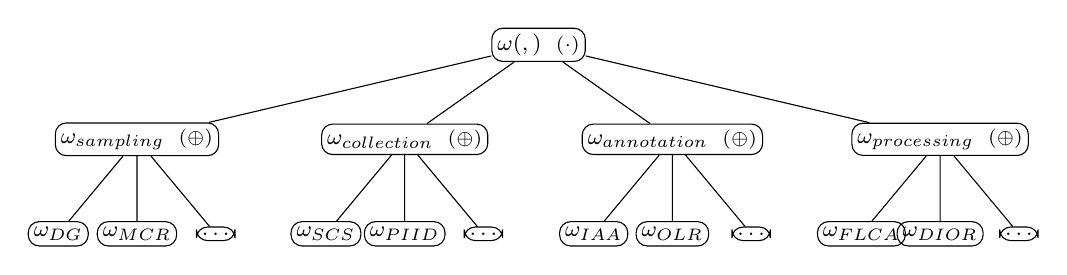
\begin{tikzpicture}[
  level distance=12mm,
  level 1/.style={sibling distance=34mm},
  level 2/.style={sibling distance=10mm},
  every node/.style={draw, rectangle, rounded corners, align=center,
                     inner sep=2pt, font=\footnotesize},
  edge from parent/.style={draw, thin}
]
\node {$\omega(\dataset, \propP)$ \;\scriptsize($\cdot$)}
  child { node {$\omega_{\text{sampling}}$ \;\scriptsize($\oplus$)}
    child { node {$\omega_{\text{DG}}$} }
    child { node {$\omega_{\text{MCR}}$} }
    child { node {$\dots$} }
  }
  child { node {$\omega_{\text{collection}}$ \;\scriptsize($\oplus$)}
    child { node {$\omega_{\text{SCS}}$} }
    child { node {$\omega_{\text{PIID}}$} }
    child { node {$\dots$} }
  }
  child { node {$\omega_{\text{annotation}}$ \;\scriptsize($\oplus$)}
    child { node {$\omega_{\text{IAA}}$} }
    child { node {$\omega_{\text{OLR}}$} }
    child { node {$\dots$} }
  }
  child { node {$\omega_{\text{processing}}$ \;\scriptsize($\oplus$)}
    child { node {$\omega_{\text{FLCA}}$} }
    child { node {$\omega_{\text{DIOR}}$} }
    child { node {$\dots$} }
  };
\end{tikzpicture}
\caption{Trust-expression tree for the running example $\propP$ =
  overall trustworthiness. The root combines the four stage-level opinions with conjunction
  ($\cdot$): the dataset is trustworthy only if every lifecycle stage is
  trustworthy. Each stage-level node fuses ($\oplus$) the opinions of the trust
  sources attached to it: they all provide evidence for the same stage-level
  proposition. Only two representative trust sources are shown per stage; the
  catalogue is given in \cref{tab:dataset-trust:catalogue}.}
\label{fig:trust_expression_tree_dataset}
\end{figure}

\paragraph{The trust-source catalogue.}
\cref{tab:dataset-trust:catalogue} is the catalogue from which the leaves of the tree are selected. It is organized by lifecycle stage and, within each stage, by \emph{risk category}: a named failure mode of that stage (e.g., temporal bias in sampling, measurement bias in collection). Each risk category is tagged with the property it threatens, so that the property axis $\propP$ can be used to filter the table, and each trust source is tagged with the granularity at which it naturally operates. The risk categories and the trust sources were assembled from the dataset-quality and bias literature: the bias taxonomy of Mehrabi et al.~\cite{10.1145/3457607} and of Suresh and Guttag~\cite{Suresh_2021} provided the risk categories, while the documentation practices of Datasheets~\cite{gebru2018datasheets} and Data Cards~\cite{Pushkarna2022DataCP} suggested which diagnostics are realistically available at each stage. The catalogue is deliberately \emph{not exhaustive}: it lists the trust sources considered in this thesis, and additional ones can be defined and selected when the framework is applied to a concrete system, as long as they are placed at a stage, a risk category and a granularity. \cref{fig:dataset-trust:overview} gives a graphical view of the same catalogue.

For the running example $\propP$ = overall trustworthiness, we define it as the conjunction of all properties in the catalogue: a dataset is trustworthy for training when it is representative, accurately measured and labeled, fair, privacy-compliant and free of leakage. Under this definition the whole catalogue is admissible, and the tree of \cref{fig:trust_expression_tree_dataset} is the \emph{maximal} decomposition. For a narrower $\propP$ the expression is the subtree obtained by pruning: an assessment of labeling accuracy retains only the annotation branch and, within it, only the trust sources tagged with \emph{accuracy}; a property defined exclusively at the entry level retains only the leaves whose granularity is $\eGran$.

\paragraph{Optional intermediate level.}
Between the stage level and the trust-source level, the framework can insert a third level grouping trust sources by risk category, as the layout of \cref{fig:dataset-trust:overview} suggests. This is useful when the analyst wants to require that a stage holds along several distinct risk axes \emph{simultaneously} (conjunction of risk categories, fusion within each). In this thesis we keep the two-level structure (stage $\to$ trust sources) for clarity; the three-level variant is a direct consequence of the framework and is left as an option for future instantiations. Similarly, when the way a stage is performed is itself described as a network of actors (several annotation vendors, several data providers), \acf{TNA-SL} (\cref{chap:tnasl}) can be used on the corresponding \aclu{STN} to expand the stage-level proposition into a finer expression.

\begin{figure}[!htbp]
  \centering
  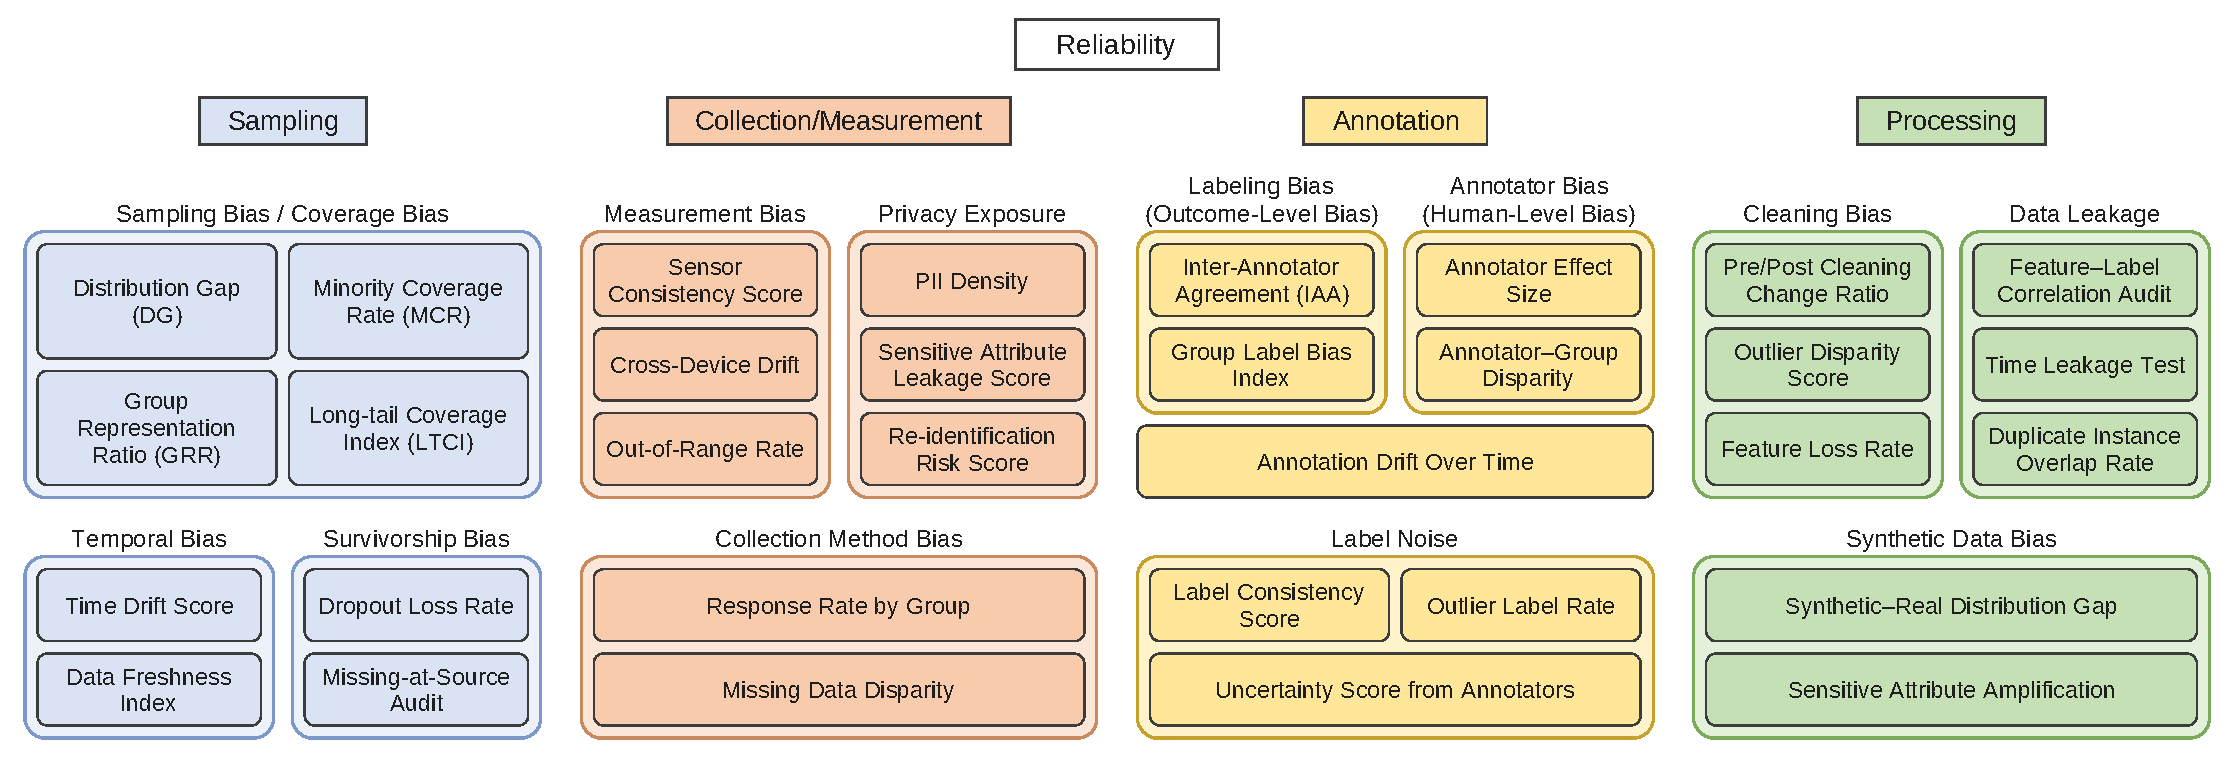
\includegraphics[width=\linewidth]{img/data/framework.pdf}
  \caption{Graphical view of the trust-source catalogue of \cref{tab:dataset-trust:catalogue}. Dataset trustworthiness is decomposed into lifecycle stages (sampling, collection, annotation, processing); within each stage, trust sources are grouped by risk category. The property each risk category informs is given in \cref{tab:dataset-trust:catalogue}. Evidence is aggregated under uncertainty using \ac{SL}.}
  \label{fig:dataset-trust:overview}
\end{figure}

\begin{table}[!htbp]
  \centering
  \footnotesize
  \setlength{\tabcolsep}{4pt}
  \renewcommand{\arraystretch}{1.12}
  \begin{tabular}{@{}lllll@{}}
    \toprule
    \textbf{Stage} & \textbf{Risk category} & \textbf{Property} & \textbf{Trust source} & \textbf{Gran.} \\
    \midrule
    \multirow{8}{*}{Sampling}
      & Sampling/Coverage Bias & Represent. & Distribution Gap (DG)               & $\dGran$ \\
      &                        &            & Minority Coverage Rate (MCR)        & $\dGran$ \\
      &                        &            & Group Representation Ratio (GRR)    & $\dGran$ \\
      &                        &            & Long-Tail Coverage Index (LTCI)     & $\dGran$ \\
      & Temporal Bias          & Represent. & Time Drift Score (TDS)              & $\dGran$ \\
      &                        &            & Data Freshness Index (DFI)          & $\dGran$ \\
      & Survivorship Bias      & Represent. & Dropout Loss Rate (DLR)             & $\dGran$ \\
      &                        &            & Missing-at-Source Audit (MSA)       & $\dGran$ \\
    \midrule
    \multirow{8}{*}{Collection}
      & Measurement Bias       & Accuracy   & Sensor Consistency Score (SCS)      & $\fGran$ \\
      &                        &            & Cross-Device Drift (CDD)            & $\fGran$ \\
      &                        &            & Out-of-Range Rate (ORR)             & $\eGran$/$\fGran$ \\
      & Privacy Exposure       & Privacy    & PII Density (PIID)                  & $\dGran$/$\fGran$ \\
      &                        &            & Sensitive Attribute Leakage (SALS)  & $\fGran$ \\
      &                        &            & Re-identification Risk (RRS)        & $\eGran$ \\
      & Collection Method Bias & Fairness   & Response Rate by Group (RRG)        & $\dGran$ \\
      &                        &            & Missing Data Disparity (MDD)        & $\dGran$ \\
    \midrule
    \multirow{9}{*}{Annotation}
      & Labeling Accuracy/Bias & Accuracy   & Inter-Annotator Agreement (IAA)     & $\eGran$ \\
      &                        & Fairness   & Group Label Bias Index (GLBI)       & $\dGran$ \\
      &                        & Accuracy   & Annotation Drift Over Time (ADT)    & $\dGran$ \\
      & Annotator Bias         & Fairness   & Annotator Effect Size (AES)         & $\dGran$ \\
      &                        &            & Annotator-Group Disparity (AGD)     & $\dGran$ \\
      &                        &            & Annotator Drift Over Time (ADOT)    & $\dGran$ \\
      & Label Noise            & Accuracy   & Label Consistency Score (LCS)       & $\eGran$ \\
      &                        &            & Outlier Label Rate (OLR)            & $\eGran$ \\
      &                        &            & Uncertainty Score from Annotators (USA) & $\eGran$ \\
    \midrule
    \multirow{8}{*}{Processing}
      & Cleaning Bias          & Fairness   & Pre/Post Cleaning Change Ratio (PCCR) & $\dGran$ \\
      &                        &            & Outlier Disparity Score (ODS)         & $\eGran$ \\
      &                        &            & Feature Loss Rate (FLR)               & $\fGran$ \\
      & Data Leakage           & Integrity  & Feature--Label Correlation Audit (FLCA) & $\fGran$ \\
      &                        &            & Time Leakage Test (TLT)               & $\dGran$ \\
      &                        &            & Duplicate Instance Overlap Rate (DIOR) & $\eGran$ \\
      & Synthetic Data Bias    & Represent. & Synthetic--Real Distribution Gap (SRDG) & $\dGran$ \\
      &                        &            & Sensitive Attribute Amplification (SAA) & $\fGran$ \\
    \bottomrule
  \end{tabular}
  \caption{Trust-source catalogue, grouped by lifecycle stage and risk category, with the property each risk category informs (Represent.\ = representativeness; Integrity = freedom from leakage) and the typical granularity ($\dGran$ = dataset, $\eGran$ = entry, $\fGran$ = feature). Risk categories follow the bias taxonomies of~\cite{10.1145/3457607,Suresh_2021}; the trust sources are adapted from the dataset-documentation practices of~\cite{gebru2018datasheets,Pushkarna2022DataCP}. The catalogue is extensible; \cref{sec:dataset-trust:applications:compas} defines the trust sources actually used in this thesis.}
  \label{tab:dataset-trust:catalogue}
\end{table}

\subsection{Phase~II --- Quantification of the Leaves}
\label{sec:dataset-trust:framework:phase2}
Phase~I has fixed the structure of the assessment. What remains is the quantification of each leaf, which proceeds in two steps: (1) designing, for each trust source, how its output becomes positive and negative evidence, and (2) turning evidence into a subjective opinion.

\subsubsection{From trust-source outputs to evidence}
\label{sec:dataset-trust:formal:evidence}
As in \cref{sec:evidence_collection}, how the output of a trust source is turned into evidence is part of the design of that trust source, and the framework does not prescribe it. The only contract is that step (1) delivers, for each leaf, a pair of non-negative evidence counts $(r, s)$ whose meaning is fixed by the property $\propP$ (what counts for and against the proposition), and that the mapping and its hyperparameters are reported with the assessment. The output of a trust source may be a scalar, a distribution, a set of per-unit outcomes or an audit result; the applications of this chapter show several such mappings (\cref{sec:dataset-trust:applications:gtsrb,sec:dataset-trust:applications:cifar10h}). What follows is the \emph{default recipe} for the most common case, a scalar metric, which is the one used in the \ac{COMPAS} application.

\paragraph{Default recipe for scalar metrics.}
Trust sources return values on very different scales (a rate in $[0,1]$, a \ac{KL} divergence, a ratio, a number of days). To make them comparable, each value $m$ is first mapped to a normalized \emph{quality score} $q_m \in [0,1]$, where $q_m$ close to one means strong support for the stage-level proposition and $q_m$ close to zero means evidence against it. Two linear ramps cover the two possible directions (\cref{fig:dataset-trust:ramps}).

For trust sources where \emph{lower} values are better (error rates, divergences, leakage scores):
\begin{equation}
q_m = \max\!\left(0,\, 1 - \frac{m}{\tau_m}\right),
\label{eq:dataset-trust:q-low}
\end{equation}
where $\tau_m > 0$ is a tolerance threshold: $q_m = 1$ when $m = 0$, $q_m = 0$ once $m$ reaches $\tau_m$, and values beyond $\tau_m$ are clamped at zero since further degradation adds nothing useful. The choice of $\tau_m$ is the operational definition of ``how bad is too bad'' for this trust source. A lower bound is unnecessary because such values are non-negative and zero is always ideal.

For trust sources where \emph{higher} values are better (coverage rates, freshness indices):
\begin{equation}
q_m = \max\!\left(0,\, \min\!\left(1,\,
        \frac{m - A_m}{L_m - A_m}\right)\right),
\label{eq:dataset-trust:q-high}
\end{equation}
where $A_m$ is the value below which the trust source gives no support at all and $L_m$ the value at which support saturates. Two thresholds are needed here because the ``good'' region has both a floor and a saturation point.

\begin{figure}[!htbp]
  \centering
  \begin{subfigure}{0.46\textwidth}
    \centering
    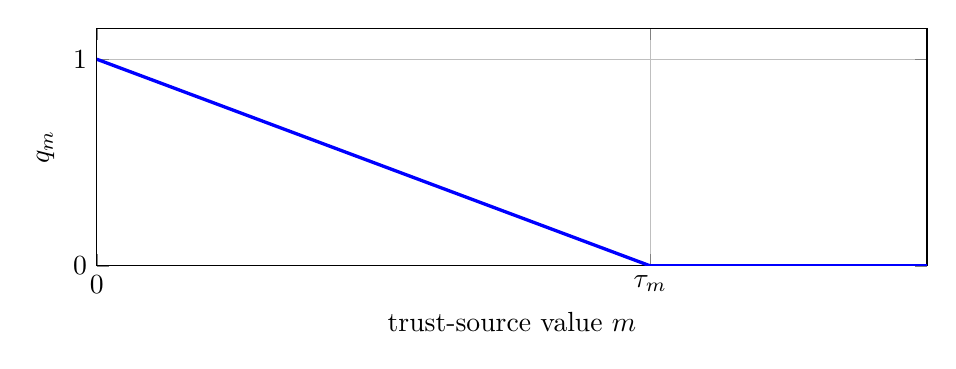
\begin{tikzpicture}
      \begin{axis}[width=\linewidth, height=4.6cm, xmin=0, xmax=1.5, ymin=0, ymax=1.15,
        xlabel={trust-source value $m$}, ylabel={$q_m$}, xtick={0,1}, xticklabels={$0$,$\tau_m$},
        ytick={0,1}, grid=major, every axis plot/.append style={very thick}]
        \addplot[blue] coordinates {(0,1) (1,0) (1.5,0)};
      \end{axis}
    \end{tikzpicture}
    \caption{Lower is better, \cref{eq:dataset-trust:q-low}.}
  \end{subfigure}
  \hfill
  \begin{subfigure}{0.46\textwidth}
    \centering
    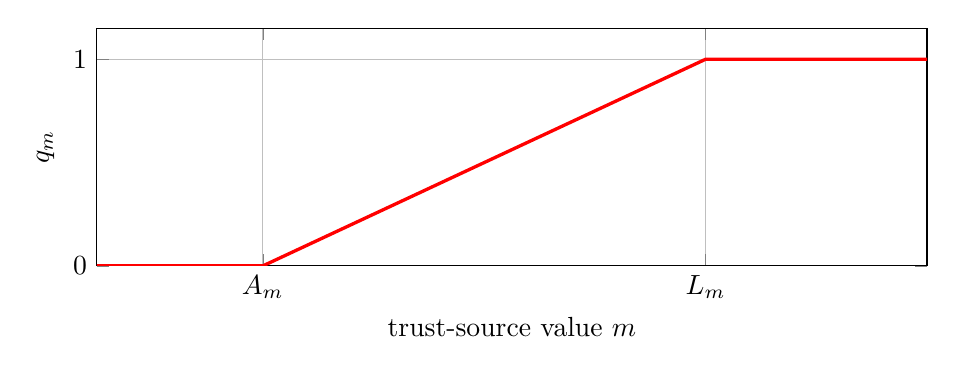
\begin{tikzpicture}
      \begin{axis}[width=\linewidth, height=4.6cm, xmin=0, xmax=1.5, ymin=0, ymax=1.15,
        xlabel={trust-source value $m$}, ylabel={$q_m$}, xtick={0.3,1.1}, xticklabels={$A_m$,$L_m$},
        ytick={0,1}, grid=major, every axis plot/.append style={very thick}]
        \addplot[red] coordinates {(0,0) (0.3,0) (1.1,1) (1.5,1)};
      \end{axis}
    \end{tikzpicture}
    \caption{Higher is better, \cref{eq:dataset-trust:q-high}.}
  \end{subfigure}
  \caption{The two normalization ramps mapping a trust-source value $m$ to a quality score $q_m \in [0,1]$.}
  \label{fig:dataset-trust:ramps}
\end{figure}

The quality score is then converted into positive and negative evidence counts:
\begin{equation}
r_m = K_m \, q_m, \qquad s_m = K_m \, (1 - q_m),
\label{eq:dataset-trust:evidence-counts}
\end{equation}
where $K_m$ is an \emph{evidence-strength} parameter fixing the total amount of evidence the trust source is assumed to provide ($r_m + s_m = K_m$). A large $K_m$ means the analyst takes the trust source seriously; a small $K_m$ means it is weak or only indicative. Under \ac{BPQ} with prior weight $W$ (below), a single trust source contributes residual uncertainty $u = W/(W + K_m)$, so $K_m$ also controls how much uncertainty one trust source leaves.

Trust sources that already produce \emph{counts} (a number of agreeing annotators, a number of contributors above a threshold, a number of classes inside a tolerance zone) skip the ramp: their counts are used directly as $(r, s)$. The \ac{GTSRB} and CIFAR-10H applications are of this kind.

\subsubsection{From evidence to opinions}
\label{sec:dataset-trust:formal:quantification}
The three quantification schemes of \cref{sec:trust_quant_model} map $(r, s)$ to an opinion $(b, d, u)$; we only recall their intuition here and refer to \cref{eq:baseline_quant_meth,eq:weight_quant_meth,eq:constant_quant_meth} for the formulas.
\begin{itemize}
  \item \textbf{\acf{BPQ}}: $u = W/(W + r + s)$, so uncertainty shrinks as evidence accumulates, at a rate set by the prior weight $W$. It is the default when the trust source returns a value with no indication of its own confidence.
  \item \textbf{\acf{EWQ}}: each piece of evidence carries its own weight $w$, so the \emph{quality} of the evidence, not only its amount, drives the uncertainty. It applies when the trust source provides a per-observation confidence (e.g., an annotator's self-reported confidence).
  \item \textbf{\acf{CUQ}}: the uncertainty is fixed externally to a value $U$ (by domain policy or by trust-source metadata) and the remaining mass $1-U$ is split between belief and disbelief in proportion to $r$ and $s$. It applies when the confidence of the assessment is bounded by something other than the number of observations.
\end{itemize}
The analyst picks one scheme per leaf according to the nature of the evidence the trust source produces; the applications exercise BPQ and CUQ, and identify where EWQ would apply (\cref{sec:dataset-trust:applications:gtsrb:method2,sec:dataset-trust:applications:cifar10h}).

\subsubsection{Setting the hyperparameters}
\label{sec:dataset-trust:framework:hyperparameters}
Phase~II introduces four kinds of hyperparameters: the normalization thresholds ($\tau_m$, or $A_m$ and $L_m$), the evidence strength $K_m$, the prior weight $W$, and, under \ac{CUQ}, the fixed uncertainty $U$. Their values are part of the assessment and must be reported with it. We recommend the following.
\begin{itemize}
  \item \textbf{Thresholds.} They encode what the application considers acceptable and are therefore \emph{domain} decisions, not statistical ones. The most principled sources are regulatory or contractual requirements (e.g., a maximum re-identification risk, a minimum coverage of a protected group) and expert elicitation, which is standard practice in risk assessment and is how acceptance criteria are set in safety and conformity assessment. When neither is available, a practical fallback is the empirical distribution of the trust-source value across datasets known to be acceptable, from which $\tau_m$ (or $A_m$, $L_m$) is read as a quantile. Sensitivity analysis, as done for the tolerance $\eta$ in \cref{sec:dataset-trust:applications:gtsrb:eval}, should accompany any threshold choice: a threshold inside a region where the opinion is stable is defensible even if it was elicited.
  \item \textbf{Evidence strength $K_m$.} A uniform value is appropriate when there is no prior reason to weight one trust source over another; this is what we do in the \ac{COMPAS} application. Differing authority (an audited metric versus a heuristic) is expressed by setting $K_m$ proportionally.
  \item \textbf{Prior weight $W$.} $W = 2$ is the non-informative default of \cref{chap:rw}; a larger $W$ (5--10) is preferable for noisy trust sources, since it slows the decrease of uncertainty.
\end{itemize}

\subsection{Phase~III --- Expression Evaluation}
\label{sec:dataset-trust:framework:phase3}
Once the leaf opinions are quantified, the expression assembled in Phase~I is evaluated bottom-up with the \ac{SL} operators: fusion within each stage (\cref{eq:dataset-trust:metric-aggregation}), conjunction across stages (\cref{eq:dataset-trust:lifecycle-decomposition}). The result is an opinion on the original proposition together with the stage-level opinions, which are kept as part of the output because they carry the diagnostic information (which stage is weak, and whether it is weak because of negative evidence or because of missing evidence).

\subsection{Cross-granularity composition of trust sources}
\label{sec:dataset-trust:formal:granularity}

The granularity $\propG$ of the property being assessed and the granularity of the trust sources used to assess it are two related choices. A dataset-level property does not need to be evaluated only by dataset-level trust sources; it can equally be assessed by aggregating evidence collected at finer granularities. Similarly, an entry-level property can rely on feature-level evidence about the columns that compose the entry. Trust sources at a finer granularity than the property can be used, as long as their evidence is aggregated up to the level at which the property is defined. The composition flows upward along the granularity hierarchy:
\[\fGran \to \eGran \to \dGran\]

Two complementary mechanisms support this upward aggregation.
\begin{itemize}
    \item \textbf{Opinion composition.} The property is decomposed unit by unit at the finer granularity. Each unit (feature or entry) is assigned a trust source, which produces an \ac{SL} opinion for that unit. The per-unit opinions are then combined into a coarser-grained opinion using \ac{SL} fusion operators, reflecting the assumption that the units jointly constitute the higher-level object.

    \item \textbf{Evidence lifting.} A single trust source produces per-unit outcomes at the finer granularity. A threshold is applied to each outcome: units that satisfy the property contribute positive evidence, and those that do not contribute negative evidence. The resulting counts are then quantified with one of the three schemes of \cref{sec:dataset-trust:formal:quantification} to produce a single opinion at the coarser level.
\end{itemize}
\noindent An entry is a structured combination of features. Both mechanisms can be applied at any level of the granularity hierarchy, moving evidence upward from features to entries, from entries to the dataset, or directly from features to the dataset. The two can also be chained, for instance by first composing feature-level opinions into per-entry opinions and then lifting those to the dataset level. Because entry- and feature-level trust sources operate on one entry at a time, they apply unchanged to a single input presented at inference time; this is how \cref{chap:patas} obtains input-level opinions.

\subsection{Overview of the Applications}
\label{sec:dataset-trust:framework:applications-overview}
The next three sections instantiate the framework. They cover part of the design space (\cref{tab:dataset-trust:applications-summary}): they were selected to show different properties, different stages and different granularities, and to serve three distinct purposes, which we state up-front because they determine how the results should be read.

\begin{description}
  \item[\ac{COMPAS} (\cref{sec:dataset-trust:applications:compas}) --- an \emph{illustration} of multi-stage composition.]\hfill\\ A tabular dataset for which trust sources exist at all four lifecycle stages. There is no ground truth for ``overall trustworthiness'', so this application does not evaluate the framework; it walks through Phases~I--III end-to-end on a real dataset and shows what the stage-level opinions add over a scalar score. Research question: \emph{can the framework compose heterogeneous stage-level evidence into a dataset-level opinion that remains traceable to the stage that weakened it?}
  \item[\ac{GTSRB} (\cref{sec:dataset-trust:applications:gtsrb}) --- an \emph{evaluation} of two trust sources for one property.]\hfill\\ An image-classification dataset whose class imbalance is known and controllable, so the trust opinion can be compared against a ground truth (the class distribution) and against its downstream effect (the accuracy gap of a trained \ac{CNN}). Research question: \emph{do the trust opinions track a known imbalance and its effect on the model, both when the global distribution is observable (centralized) and when it is not (federated)?}
  \item[CIFAR-10H (\cref{sec:dataset-trust:applications:cifar10h}) --- an \emph{evaluation} at the entry level.]\hfill\\ An image dataset in which every image carries about fifty independent human labels, so per-entry disagreement is directly observable. Research question: \emph{do per-entry opinions derived from annotator agreement identify genuinely ambiguous items, and does their uncertainty respond correctly to the amount of annotation?}
\end{description}
Each application opens with its position in the design space, introduces its dataset, states the trust proposition, and closes with what the example showed. The applications are presented multi-stage first (the general case), then sampling (dataset level), then annotation (entry level).

\FloatBarrier

% ==============================================================
\section{Multi-stage Assessment: COMPAS}
\label{sec:dataset-trust:applications:compas}
\begin{mdframed}[backgroundcolor=blue!4, linewidth=0pt]
\textbf{Position in the design space.}

$\propP$ = overall trustworthiness (conjunction of representativeness, accuracy, fairness, privacy and integrity, \cref{sec:dataset-trust:framework:phase1});\

$\propS = \{\textsc{sampling}, \textsc{collection}, \textsc{annotation},
        \textsc{processing}\}$;\

$\propG$ = dataset;\

\textbf{Quantification:} \ac{BPQ}.

\textbf{Purpose:} illustration of multi-stage composition (original to this dissertation).
\end{mdframed}

This application walks through the three phases of the framework end-to-end on a real dataset. Its purpose is to show how heterogeneous evidence from the four lifecycle stages is composed into one dataset-level opinion while remaining traceable to the stage that produced it; it is not an evaluation against a ground truth, since no reference value of ``overall trustworthiness'' exists for a dataset\footnote{The raw values reported in this section are computed with the implementation developed for this chapter, available at \url{https://github.com/Ouatt-Isma/-Trustworthiness-of-AI-Training-Dataset}. The repository documents the exact computation of every trust source; this section defines them at the level needed to follow the assessment.}.

\paragraph{Dataset.}
\ac{COMPAS} is a commercial recidivism risk-assessment tool used by US courts. The dataset used here is the ``two-year'' file released by ProPublica in its \emph{Machine Bias} investigation~\cite{angwin2016machine}: records of $7{,}214$ defendants screened with \ac{COMPAS} in Broward County, Florida, between 2013 and 2014, joined with public criminal records covering the following two years. After the standard ProPublica filtering (charge date within 30 days of the screening date, valid recidivism record), $6{,}172$ defendants remain. Each record contains demographic attributes (sex, age, age category, race), criminal history (number of prior offenses and juvenile counts), the current charge (degree, description, jail entry and exit dates), the \ac{COMPAS} risk decile (\texttt{decile\_score}, 1--10), direct identifiers (name, date of birth), and the label \texttt{two\_year\_recid} (whether the defendant re-offended within two years; $45.5\%$ positives). The dataset is $51.4\%$ African-American and $34.1\%$ Caucasian, far from the general population. It is a widely studied fairness benchmark: ProPublica showed that the \ac{COMPAS} scores have markedly different false-positive rates across racial groups. It was chosen because it is tabular, with demographic attributes, dates, direct identifiers and an outcome label, so that trust sources of all four lifecycle stages can be computed, and because its construction is publicly documented~\cite{angwin2016machine}.

\paragraph{Trust proposition and expression.}
The proposition is ``the \ac{COMPAS} dataset is trustworthy for training a recidivism classifier''. Phase~I decomposes it along the four stages as in \cref{eq:dataset-trust:lifecycle-decomposition}; at each stage we attach the trust sources of \cref{tab:dataset-trust:catalogue} that can be computed from the available columns, all at dataset granularity. Note that in \ac{COMPAS} the ``annotation'' stage is the recording of the recidivism outcome from court records, not a human labeling campaign: there are no multiple annotators, so the only applicable annotation trust source is the group-label bias index. \cref{tab:dataset-trust:compas-sources} defines the thirteen trust sources retained, as computed on \ac{COMPAS}, together with the threshold used for each.

\begin{table}[!htbp]
  \centering
  \small
  \renewcommand{\arraystretch}{1.15}
  \begin{tabular}{@{}llp{7.9cm}l@{}}
    \toprule
    \textbf{Stage} & \textbf{Source} & \textbf{Definition on COMPAS} & \textbf{Threshold} \\
    \midrule
    \multirow{9}{*}{Sampling}
      & DG   & \ac{KL} divergence between the racial distribution of the dataset and a census-based reference distribution of the general population ($\downarrow$). & $\tau=0.30$ \\
      & MCR  & Ratio of the frequency of African-Americans in the dataset to their frequency in the reference population ($\uparrow$). & $A=0.5$, $L=1$ \\
      & LTCI & Fraction of rare charge descriptions ($<1\%$ of records) that still occur in the most recent half of the records ($\uparrow$). & $A=0.3$, $L=1$ \\
      & DFI  & Mean freshness of records, decaying linearly from 1 at the reference date to 0 one year earlier; the reference date is the latest \texttt{c\_jail\_in} ($\uparrow$). & $A=0$, $L=1$ \\
      & MSA  & Fraction of records missing at least one essential field (race, sex, age, priors, decile score, label) ($\downarrow$). & $\tau=0.10$ \\
    \midrule
    \multirow{9}{*}{Collection}
      & ORR  & Fraction of decile scores outside the valid range $[1,10]$ ($\downarrow$). & $\tau=0.05$ \\
      & MDD  & Largest difference in missingness rate of the essential fields between racial groups ($\downarrow$). & $\tau=0.20$ \\
      & PIID & Fraction of columns that are direct identifiers (name, first, last, dob) ($\downarrow$). & $\tau=0.001$ \\
      & SALS & In-sample accuracy of a logistic regression predicting race from the non-sensitive features (age, priors, juvenile counts, decile score) ($\downarrow$). & $\tau=0.70$ \\
      & RRS  & Mean inverse size of the anonymity set defined by the quasi-identifiers (sex, race, age category), i.e., $k$-anonymity risk ($\downarrow$). & $\tau=0.50$ \\
    \midrule
    Annotation
      & GLBI & \ac{KL} divergence between the label distributions of African-American and Caucasian defendants ($\downarrow$). & $\tau=0.20$ \\
    \midrule
    \multirow{2}{*}{Processing}
      & DIOR & Fraction of exact duplicate rows ($\downarrow$). & $\tau=0.01$ \\
      & FLCA & Maximum absolute Pearson correlation between any numeric feature and the label, a shortcut/leakage indicator ($\downarrow$). & $\tau=0.60$ \\
    \bottomrule
  \end{tabular}
  \caption{Trust sources used in the \ac{COMPAS} assessment. $\downarrow$: lower is better, normalized with \cref{eq:dataset-trust:q-low}; $\uparrow$: higher is better, normalized with \cref{eq:dataset-trust:q-high}. Evidence strength $K_m = 2$ and prior weight $W = 2$ for all trust sources.}
  \label{tab:dataset-trust:compas-sources}
\end{table}

The thresholds were set as follows\footnote{We stress that these values are illustrative. $\tau_{\text{DG}} = 0.30$ tolerates at most $0.30$ nats of divergence from the reference population; $A_{\text{MCR}} = 0.50$ requires the minority group to be represented at least at half its population rate, with parity ($L = 1$) as the ideal; $\tau_{\text{PIID}} = 0.001$ effectively requires that no direct identifier be present. In a deployment they would be elicited from the domain expert or derived from the applicable requirements, as discussed in \cref{sec:dataset-trust:framework:hyperparameters}. Whether this is practical depends on the setting: for regulated domains such as criminal justice or medical devices, acceptance criteria of this kind already have to be documented, so the elicitation cost is incurred anyway; the framework simply makes them explicit inputs of the assessment.}: for each trust source we asked what value a domain expert would consider clearly unacceptable and, for higher-is-better sources, what value would be ideal. All trust sources use the same evidence strength $K_m = 2$ (no prior reason to weight one over another) and the non-informative prior weight $W = 2$.

\subsection{Stage quantification on COMPAS}
\label{sec:dataset-trust:applications:compas:stages}

 \paragraph{Sampling stage.}
The sampling-stage proposition is \emph{``the sampling stage of the \ac{COMPAS} dataset is trustworthy.''} Five trust sources contribute evidence: DG, MCR, LTCI, DFI and MSA. We walk through this stage in detail to illustrate Phase~II; for the sake of brevity, we only summarize the final assessment results of the other three stages (\cref{tab:dataset-trust:compas}).

\subparagraph{Step~1: Normalizing the values.}
The observed values are
\[
\text{DG} = 0.432,\quad \text{MCR} = 3.597,\quad
\text{LTCI} = 0.657,\quad \text{DFI} = 0.100,\quad
\text{MSA} = 0.000.
\]
DG and MCR both compare the dataset to the reference population: the divergence is large (DG $= 0.432 > \tau_{\text{DG}}$), and African-Americans are over-represented by a factor $3.6$ with respect to their population share. DFI is computed with the dataset's own most recent record as the reference ``now''; in practice, freshness should be measured relative to the time at which the dataset is consumed, so the present convention is conservative and for illustration only. Applying \cref{eq:dataset-trust:q-low,eq:dataset-trust:q-high} with the thresholds of \cref{tab:dataset-trust:compas-sources} yields
\[
q_{\text{DG}}   = 0.000,\quad
q_{\text{MCR}}  = 1.000,\quad
q_{\text{LTCI}} = 0.510,\quad
q_{\text{DFI}}  = 0.100,\quad
q_{\text{MSA}}  = 1.000.
\]

\subparagraph{Step~2: Converting to evidence.}
With $K_m = 2$ for every trust source, $r_m = 2 q_m$ and $s_m = 2(1 - q_m)$ give
\[
\begin{aligned}
& r_{\text{DG}}   = 0.00,\ s_{\text{DG}}   = 2.00, \quad
  r_{\text{MCR}}  = 2.00,\ s_{\text{MCR}}  = 0.00, \\
& r_{\text{LTCI}} = 1.02,\ s_{\text{LTCI}} = 0.98, \quad
  r_{\text{DFI}}  = 0.20,\ s_{\text{DFI}}  = 1.80, \\
& r_{\text{MSA}}  = 2.00,\ s_{\text{MSA}}  = 0.00.
\end{aligned}
\]

\subparagraph{Step~3: Applying \ac{BPQ} and fusing.}
\ac{BPQ} with prior weight $W = 2$ gives one opinion per trust source,
\begin{align}
 \omega_{\text{DG}}   &= (0, 0.5, 0.5), \quad&
  \omega_{\text{MCR}}  &= (0.5, 0, 0.5),\\
\omega_{\text{LTCI}} &= (0.255, 0.245, 0.5), \quad&
  \omega_{\text{DFI}}  &= (0.05, 0.45, 0.5), \\
\omega_{\text{MSA}}  &= (0.5, 0, 0.5),
\end{align}
and cumulative fusion of the five opinions (\cref{eq:dataset-trust:metric-aggregation}) gives the stage-level opinion
\[
\omega_{\text{sampling}} = (0.435,\ 0.398,\ 0.167).
\]
Under \ac{BPQ}, cumulative fusion amounts to adding the evidence counts, so the stage opinion is simply $\bigl(\sum r_m,\ \sum s_m\bigr) = (5.22,\ 4.78)$ quantified with $W = 2$; this makes the stage-level result easy to audit.

\subparagraph{Interpretation.}
The opinion $(0.435,\ 0.398,\ 0.167)$ has belief and disbelief close to each other and a comparatively low uncertainty: the evidence base is large enough for the opinion to be decisive, but the evidence itself is genuinely mixed. Two trust sources contribute positive evidence: the minority coverage rate ($q_{\text{MCR}} = 1.00$) and the missing-at-source audit ($q_{\text{MSA}} = 1.00$). Two contribute negative evidence: the distribution gap ($q_{\text{DG}} = 0.00$) and the data freshness index ($q_{\text{DFI}} = 0.10$). The long-tail coverage index ($q_{\text{LTCI}} = 0.51$) is mixed. Rather than collapsing these into a single ``the sampling is good'' or ``the sampling is bad'' verdict, the framework reports both: the dataset has acceptable minority coverage and structural completeness, but exhibits a distribution gap with respect to the reference population and is stale. The two signals are surfaced separately rather than averaged away.

\begin{table}[!htbp]
  \centering
  \small
  \renewcommand{\arraystretch}{1.1}
  \begin{tabular}{@{}llrrl@{}}
    \toprule
    \textbf{Stage} & \textbf{Trust source} & \textbf{Raw} & \textbf{$q$} & \textbf{Direction / Threshold} \\
    \midrule
    \multirow{5}{*}{Sampling}
      & DG                                  & 0.432  & 0.000 & lower is better \{$\tau{=}0.3$\} \\
      & MCR(African-American)           & 3.597 & 1.000 & higher is better \{$A{=}0.5$, $L{=}1.0$\} \\
      & LTCI(c\_charge\_desc)               & 0.657  & 0.510 & higher is better \{$A{=}0.3$, $L{=}1.0$\}\\
      & DFI(c\_jail\_in)                    & 0.100 & 0.100 & higher is better \{$A{=}0$, $L{=}1.0$\} \\
      & MSA(essential\_cols)                & 0.000  & 1.000 & lower is better \{$\tau{=}0.1$\} \\
    \cmidrule(lr){2-5}
      & \multicolumn{4}{l}{\ac{BPQ} stage opinion: $(b, d, u) = (0.435,\ 0.398,\ 0.167)$\quad \{$W{=}2$\}} \\
    \midrule
    \multirow{5}{*}{Collection}
      & ORR(decile\_score)                  & 0.000  & 1.000 & lower is better \{$\tau{=}0.05$\} \\
      & MDD(by\_race)                       & 0.000  & 1.000 & lower is better \{$\tau{=}0.2$\} \\
      & PIID                                & 0.075  & 0.000 & lower is better \{$\tau{=}0.001$\} \\
      & SALS(race$\,|\,$features)           & 0.570  & 0.186 & lower is better \{$\tau{=}0.7$\} \\
      & RRS(qid$=$sex,race,age\_cat)        & 0.191  & 0.619 & lower is better \{$\tau{=}0.5$\} \\
    \cmidrule(lr){2-5}
      & \multicolumn{4}{l}{\ac{BPQ} stage opinion: $(b, d, u) = (0.467,\ 0.366,\ 0.167)$\quad \{$W{=}2$\}} \\
    \midrule
    Annotation
      & GLBI(two\_year\_recid$\,|\,$race)   & 0.036  & 0.821 & lower is better \{$\tau{=}0.2$\} \\
    \cmidrule(lr){2-5}
      & \multicolumn{4}{l}{\ac{BPQ} stage opinion: $(b, d, u) = (0.411,\ 0.089,\ 0.500)$\quad \{$W{=}2$\}} \\
    \midrule
    \multirow{2}{*}{Processing}
      & DIOR                                & 0.000  & 1.000 & lower is better \{$\tau{=}0.01$\}  \\
      & FLCA                                 & 0.291   & 0.516 & lower is better \{$\tau{=}0.6$\}  \\
    \cmidrule(lr){2-5}
      & \multicolumn{4}{l}{\ac{BPQ} stage opinion: $(b, d, u) = (0.505,\ 0.161,\ 0.333)$\quad \{$W{=}2$\}} \\
    \bottomrule
  \end{tabular}
  \caption{Raw values, quality scores and stage-level opinions for \ac{COMPAS} ($K_m = 2$ for every trust source). Each stage is quantified independently with \cref{eq:dataset-trust:q-low,eq:dataset-trust:q-high} and \ac{BPQ}; the dataset-level opinion is obtained by the cross-stage conjunction of \cref{eq:dataset-trust:lifecycle-decomposition}.}
  \label{tab:dataset-trust:compas}
\end{table}

\paragraph{Collection stage.}
The collection stage produces a more balanced assessment, with belief $b = 0.467$, disbelief $d = 0.366$ and uncertainty $u = 0.167$. The measurement-integrity trust sources, out-of-range rate ($q = 1.000$) and missing-data disparity ($q = 1.000$), contribute positive evidence: the decile scores are all in range and missingness does not differ across racial groups. The privacy trust sources, however, contribute substantial negative evidence: the file ships with direct identifiers (\ac{PII} density $q = 0.00$), race can be predicted from the non-sensitive features with $57\%$ accuracy (sensitive-attribute leakage $q = 0.186$), and the quasi-identifiers leave a non-negligible re-identification risk ($q = 0.619$). Privacy is part of the property being assessed (overall trustworthiness, as defined in \cref{sec:dataset-trust:framework:phase1}, includes privacy compliance), so this evidence legitimately lowers the collection-stage opinion; an analyst assessing a narrower property such as measurement accuracy would prune the privacy trust sources and obtain a clearly positive collection-stage opinion. The resulting opinion reflects a trade-off between accurate measurement and privacy exposure rather than a clear conclusion.

\paragraph{Annotation stage.}
The annotation stage is assessed with a single trust source, the group-label bias index, whose value ($0.036$ nats) is well within tolerance and gives $q = 0.821$. The stage-level opinion is $(b, d, u) = (0.411, 0.089, 0.500)$: the lowest belief of the four stages. This low belief should not be read as ``the annotation is not trustworthy'': disbelief is correspondingly low, and the dominant mass is uncertainty. The framework is reporting that, with only one trust source available ($r + s = K_m = 2$), it does not have enough evidence to be confident in either direction. This is qualitatively different from the sampling-stage opinion, which has comparable belief but reached it through balanced positive and negative evidence rather than through absent evidence.

\paragraph{Processing stage.}
The processing stage yields the strongest signal, with belief $b = 0.505$, disbelief $d = 0.161$ and uncertainty $u = 0.333$. The absence of duplicate rows provides strong positive evidence ($q = 1.00$), and the feature--label correlation audit ($q = 0.516$, maximum correlation $0.29$ with \texttt{priors\_count}) is mildly positive. Residual uncertainty remains because only two processing-stage diagnostics can be computed on a dataset whose cleaning history is not available.

\paragraph{Cross-stage rollup.}
The four stage-level opinions are combined into a dataset-level trustworthiness opinion by the cross-stage conjunction of \cref{eq:dataset-trust:lifecycle-decomposition}:
\[
\omega_{\dataset}
= \omega_{\text{sampling}} \cdot
  \omega_{\text{collection}} \cdot
  \omega_{\text{annotation}} \cdot
  \omega_{\text{processing}} = (0.12,\ 0.71,\ 0.17).
\]
The result is dominated by disbelief: the evidence accumulated across the four stages points against the trustworthiness of the dataset rather than for it. This is a direct consequence of conjunction: a single stage with high disbelief is sufficient to pull the combined opinion toward disbelief, regardless of how well the other stages perform. Here the collection and sampling stages, both carrying substantial disbelief, are the primary drivers. The residual uncertainty $u = 0.17$ mainly reflects the limited diagnostic coverage of the annotation stage.

\paragraph{What this example showed.}
Read together with \cref{tab:dataset-trust:compas}, the rollup preserves three pieces of information that a scalar quality score would collapse: \emph{which} stage carries the strongest negative signal (collection, through privacy exposure), \emph{which} stage merely lacks evidence (annotation, with $u = 0.50$ from a single trust source), and how the stages compare quantitatively. These correspond to two qualitatively different actions for an auditor: collecting more representative or privacy-aware data attacks the sampling- and collection-stage disbelief, whereas gathering additional annotation-stage diagnostics reduces the annotation-stage uncertainty. The example also showed the two properties of the quantification that make the result auditable: under \ac{BPQ}, fusion within a stage is a sum of evidence counts, and every hyperparameter ($\tau$, $A$, $L$, $K_m$, $W$) is an explicit, reportable input. Finally, it showed the cost of the approach: thirteen threshold values had to be set, and the assessment is only as meaningful as those choices, which is why they are reported alongside the opinions.

\FloatBarrier

% ==============================================================
\section{Sampling Stage, Dataset Level: Representativeness on \acs{GTSRB}}
\label{sec:dataset-trust:applications:gtsrb}

\begin{mdframed}[backgroundcolor=blue!4, linewidth=0pt]
\textbf{Position in the design space.}

$\propP$ = representativeness (class balance);\quad
$\propS = \{\textsc{sampling}\}$;\quad $\propG$ = dataset;\

\textbf{Quantification:} \ac{CUQ} (global-distribution trust source), \ac{BPQ} (local-entropy trust source).\quad

\textbf{Purpose:} evaluation.\quad \textbf{Published in:}~\cite{10.1007/978-3-032-19096-3_17}.
\end{mdframed}

\paragraph{Purpose and research question.}
This application evaluates the framework on one well-defined cell of the design space: the representativeness of the sampling stage, understood as class balance, at dataset granularity. Class balance was chosen because it is a property for which a \emph{ground truth} exists (the class distribution is directly observable and can be manipulated) and whose downstream effect is measurable (the accuracy of a classifier on under-represented classes). The research question is: \emph{do the trust opinions produced by the framework track a known class imbalance and its effect on the trained model, both when the global class distribution is observable (centralized setting) and when it is not (federated setting)?} The federated setting is motivated by the \ac{CCAM} use case of this thesis, in which several \acp{OEM} contribute driving data to a shared training set without disclosing their raw data. It leads to two different trust sources for the same proposition, which in turn exercise two of the three quantification schemes.

\paragraph{Dataset.}
The \acf{GTSRB}~\cite{stallkamp2012man,GTSRB} contains $51{,}839$ color images of German road signs in $K = 43$ classes, split into $39{,}209$ training and $12{,}630$ test images; we resize all images to $32 \times 32$ pixels. The class distribution is documented and strongly non-uniform: the training set holds between $210$ and $2{,}250$ images per class (\cref{fig:gtsrb:distscenario1}(a)). This is not an artifact of the collection: the images were extracted from real drives, so the class frequencies reflect how often each sign occurs on the road. In particular, the fourteen triangular \emph{warning signs} (classes 18--31: dangerous curve, slippery road, pedestrians, children crossing, \dots) are among the rarest classes. Whether such an imbalance is a defect depends on the property assessed: it is acceptable, even desirable, for a proposition about representativeness of deployment-time frequencies, but for the proposition assessed here, class balance with respect to a uniform target, it is precisely what the trust opinion must detect. The documented class distribution is therefore the ground truth against which the opinions are checked, and the warning-sign group is the natural minority group on which to measure the downstream effect; the summary returns to the deployment-frequency reading.

\paragraph{Trust proposition.}
\emph{``The dataset $\dataset$ is not biased with respect to class balance.''} We treat this as a simple trust proposition at dataset level: the expression tree is a single leaf, and the application is entirely about how that leaf is quantified from two different trust sources.

To assess balance, we describe the dataset by its \emph{class-probabilities distribution}. For a classification task with $K$ classes and $N$ data points, the empirical probability of class $k$ is
\begin{equation}
P(\mathrm{Class}_k) = \frac{N_k}{N}, \qquad
\sum_{k=1}^{K} P(\mathrm{Class}_k) = 1,
\end{equation}
where $N_k$ is the number of data points belonging to class $k$. This distribution is the basic object on which both trust sources operate. A perfectly balanced dataset has all probabilities equal to $1/K$; the density of the class-probability distribution is then concentrated around $1/K$. Imbalanced datasets exhibit a wider spread. \Cref{fig:gtsrb:probability-density} illustrates this on a \emph{synthetic toy configuration}, unrelated to \ac{GTSRB}, with $K = 6$ classes and $N = 5200$ points: an imbalanced dataset with class counts $[100,\allowbreak 100,\allowbreak 1000,\allowbreak 1000,\allowbreak 1000,\allowbreak 2000]$ and a balanced one with class counts $[857,\allowbreak 857,\allowbreak 867,\allowbreak 867,\allowbreak 876,\allowbreak 876]$.

\begin{figure}[!htbp]
    \centering
    \begin{subfigure}{0.45\textwidth}
        \centering
        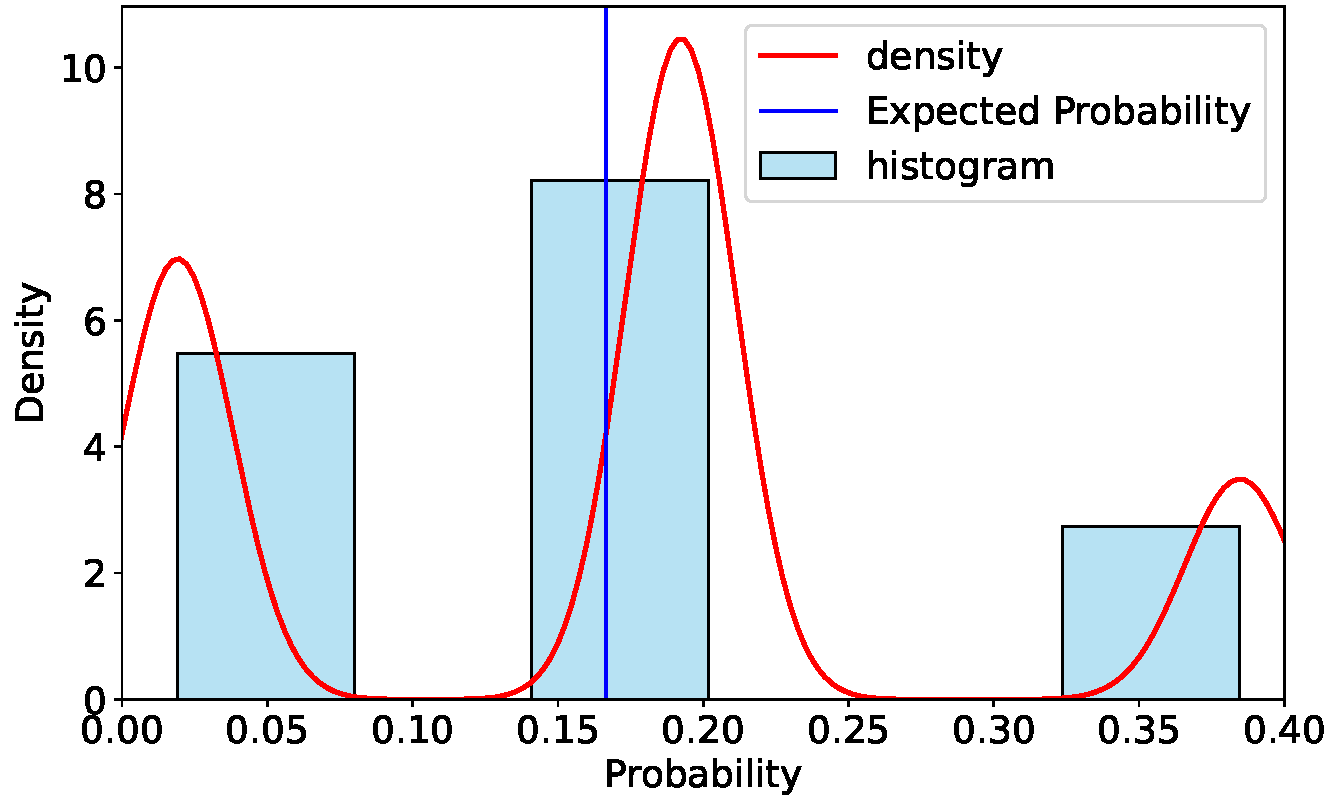
\includegraphics[width=0.95\linewidth]{img/data/imbalanced.pdf}
        \caption{Imbalanced dataset.}
    \end{subfigure}
    \begin{subfigure}{0.45\textwidth}
        \centering
        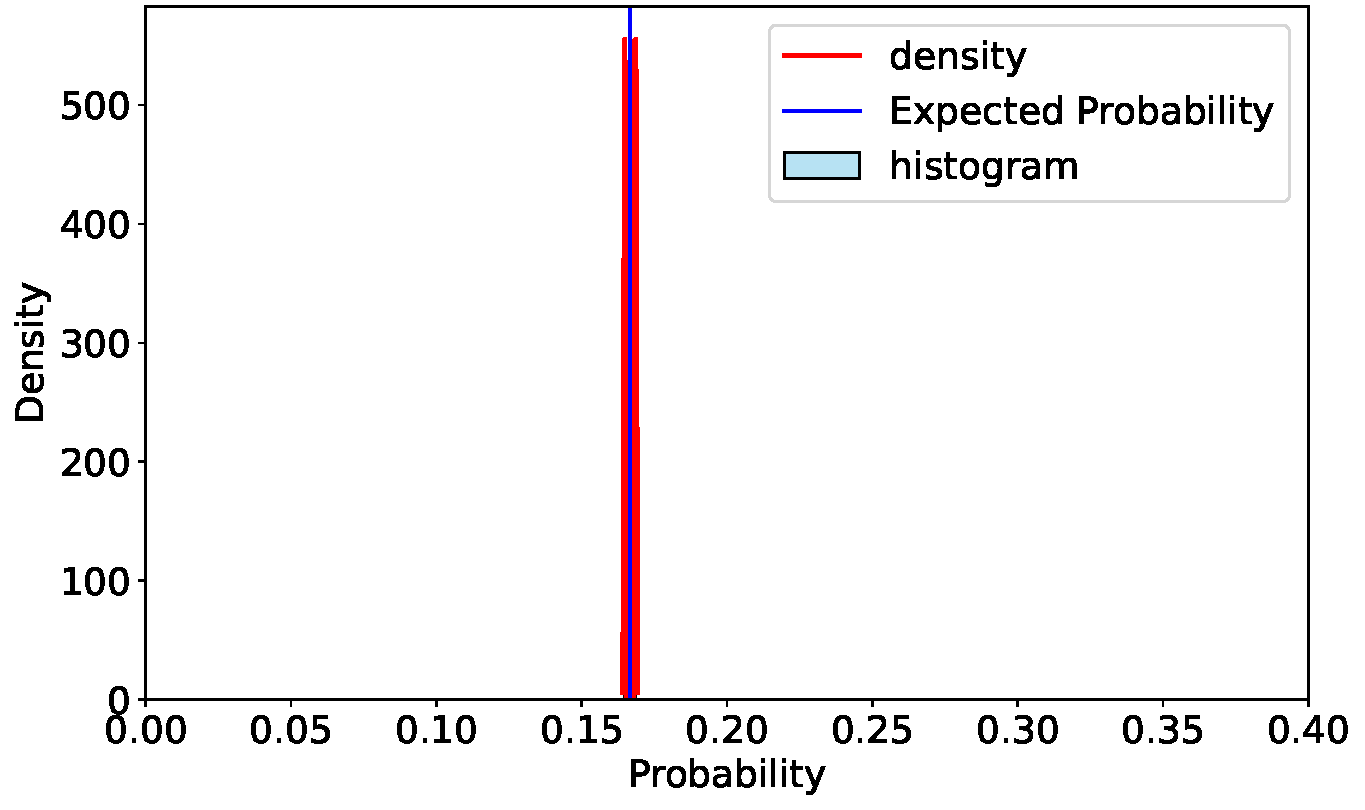
\includegraphics[width=0.95\linewidth]{img/data/balanced.pdf}
        \caption{Balanced dataset.}
    \end{subfigure}
    \caption{Density of the class-probabilities distribution for a synthetic toy example ($N = 5200$ points, $K = 6$ classes; not \ac{GTSRB}). The balanced dataset concentrates around $1/K \approx 0.167$; the imbalanced dataset shows a wider spread.}
    \label{fig:gtsrb:probability-density}
\end{figure}

\subsection{Global-distribution trust source (GD)}
\label{sec:dataset-trust:applications:gtsrb:method1}

The first trust source, which we call the \emph{global-distribution} (GD) trust source, operates on the global class-probabilities distribution directly. A class is considered \emph{balanced} when its empirical probability lies within a tolerance interval around the expected value:
\begin{equation}
P(\mathrm{Class}_k) \in
  \left[\frac{1}{K} - \eta_1,\ \frac{1}{K} + \eta_2\right].
\label{eq:gtsrb:tolerance-zone}
\end{equation}
The parameters $\eta_1, \eta_2$ control the width of the tolerance zone and play the same role as the threshold $\tau_m$ in \cref{eq:dataset-trust:q-low}: they define the boundary beyond which a class probability is considered unacceptably imbalanced. We set $\eta = \eta_1 = \eta_2$ for the experiments reported below; the impact of $\eta$ is studied in \cref{sec:dataset-trust:applications:gtsrb:eval}.

Each class provides one piece of evidence: positive if its probability falls inside the tolerance zone, negative otherwise. Normalized by $K$, positive evidence is the area under the density $f$ of the class-probabilities distribution that falls within the tolerance zone, and negative evidence the complementary area:
\begin{equation}
r = \int_{1/K - \eta_1}^{1/K + \eta_2} f(x)\, dx
  = \frac{n_t}{K},
\qquad
s = 1 - r,
\label{eq:gtsrb:method1-evidence}
\end{equation}
where $n_t$ is the number of classes whose empirical probability falls within the tolerance zone.

\paragraph{Quantification scheme: \ac{CUQ}.}
The GD evidence is naturally normalized ($r + s = 1$), so the remaining choice is how to set the uncertainty mass. The GD trust source measures balance from the empirical class-probabilities distribution, which is itself estimated from the dataset: a \emph{small} dataset gives a noisy estimate, so the trust opinion should be held with low confidence regardless of how balanced the observed distribution appears. The right notion of \emph{small} is relative to the model's data requirements, which is what \emph{sample complexity} measures in \ac{PAC} learning.

\ac{PAC} learning~\cite{valiant1984theory} asks how many training examples are needed for a learner to find, with probability at least $1 - \delta$, a hypothesis whose error is at most $\epsilon$. For a hypothesis class of \ac{VC} dimension $d$, Haussler et al.~\cite{HAUSSLER1994248} show that the required number of examples is
$\mathcal{M}(\epsilon, \delta) = \mathcal{O}\!\left(\frac{d}{\epsilon}\log\frac{1}{\delta}\right)$.
We use the leading term as a \emph{theoretical} sample complexity,
$N_s = \frac{d}{\epsilon}\log(1/\delta)$,
and set the \ac{CUQ} uncertainty from the gap between $N_s$ and the actual dataset size $N$:
\begin{equation}
U = \min\!\left(
      \max\!\left(
        \frac{\log_{10}(N_s) - \log_{10}(N)}{10},\ m_1\right),\ m_2\right),
\label{eq:gtsrb:uncertainty}
\end{equation}
where $[m_1, m_2]$ is the admissible range of uncertainty (set to $[0,1]$ in our experiments). The division by $10$ maps a gap of ten orders of magnitude to full uncertainty. \Cref{fig:gtsrb:u-vs-n} plots $U$ as a function of $N / N_s$: when $N$ is large relative to $N_s$, the dataset is sufficient for the model and the uncertainty shrinks toward zero; when $N$ is small relative to $N_s$, the assessment cannot be made with confidence regardless of how balanced the observed distribution is. Because of the logarithm, $U$ changes slowly with $N$: multiplying $N$ by ten lowers $U$ by only $0.1$.

The \ac{VC} dimension of a \ac{CNN} is not computable exactly. Following the classical bound for piecewise-linear networks, which grows with the number of parameters $P$ and layers $L$, we use the proxy $d = P \cdot L$. For the \ac{CNN} of \cref{sec:dataset-trust:applications:gtsrb:eval} ($P \approx 1.46 \times 10^{6}$, $L = 17$), $d \approx 2.5 \times 10^{7}$; with $\epsilon = 0.05$ and $\delta = 0.5$ this gives $N_s \approx 3.4 \times 10^{8}$, four orders of magnitude above the $39{,}209$ images of \ac{GTSRB}, hence $U \approx 0.39$ in all centralized experiments. This value is admittedly conservative (\ac{PAC} bounds are worst-case), which is acceptable here since $U$ is used as a \emph{relative} confidence scale across datasets of different sizes rather than as an absolute statement.

\begin{figure}[!htbp]
  \centering
  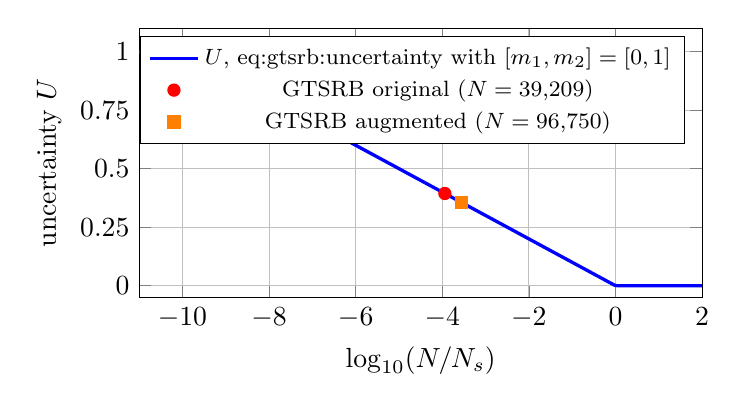
\begin{tikzpicture}
    \begin{axis}[width=0.72\linewidth, height=5cm, xmin=-11, xmax=2, ymin=-0.05, ymax=1.1,
      xlabel={$\log_{10}(N / N_s)$}, ylabel={uncertainty $U$}, grid=major,
      xtick={-10,-8,-6,-4,-2,0,2}, ytick={0,0.25,0.5,0.75,1}, legend pos=north east, legend style={font=\footnotesize}]
      \addplot[very thick, blue, domain=-11:2, samples=200] {min(max(-x/10,0),1)};
      \addlegendentry{$U$, \cref{eq:gtsrb:uncertainty} with $[m_1,m_2]=[0,1]$}
      \addplot[only marks, mark=*, mark size=2.2pt, red] coordinates {(-3.94,0.394)};
      \addlegendentry{\ac{GTSRB} original ($N = 39{,}209$)}
      \addplot[only marks, mark=square*, mark size=2.2pt, orange] coordinates {(-3.55,0.355)};
      \addlegendentry{\ac{GTSRB} augmented ($N = 96{,}750$)}
    \end{axis}
  \end{tikzpicture}
  \caption{\ac{CUQ} uncertainty of the GD trust source as a function of the ratio between the dataset size $N$ and the theoretical sample complexity $N_s$. The two markers are the datasets of Scenario~1 ($N_s \approx 3.4 \times 10^{8}$).}
  \label{fig:gtsrb:u-vs-n}
\end{figure}

Once $U$ is fixed by \cref{eq:gtsrb:uncertainty}, belief and disbelief follow from the \ac{CUQ} formula ($\gamma = (1-U)/(r+s)$, $b = \gamma r$, $d = \gamma s$).

\subsection{Local-entropy trust source (LE)}
\label{sec:dataset-trust:applications:gtsrb:method2}
In federated or collaborative settings, no single party observes the global distribution of class probabilities: each contributing node (e.g., each \ac{OEM} in a vehicular collaborative dataset) only sees its own sub-dataset. The GD trust source can still be applied if every contributor shares its class counts with an aggregator, but in privacy-sensitive settings even class counts may be considered disclosive (they reveal what a contributor's fleet has encountered). The \emph{local-entropy} (LE) trust source takes another path: each node summarizes its sub-dataset with a single scalar, and the aggregator receives only that scalar.

\paragraph{Entropy as a balance proxy.}
Each contributor $i$ computes the entropy of its local
class-probabilities distribution $P^{(i)}$:
\begin{equation}
\mathcal{H}(P^{(i)})
= -\sum_{k=1}^{K} p^{(i)}_k \log p^{(i)}_k.
\end{equation}
Entropy is maximal ($\log K$) when the local distribution is uniform and decreases as one or a few classes dominate.

Each local entropy is compared against a threshold that defines the \emph{edge of acceptable balance}. We construct an \emph{edge-acceptable} distribution $P_E$ by setting each class probability to $1/K \pm \eta$, alternating the sign so that $P_E$ sums to one (with one class set to exactly $1/K$ when $K$ is odd), and define
\begin{equation}
\mathit{Thres} = \mathcal{H}(P_E).
\end{equation}
$P_E$ is the least balanced distribution that the GD trust source would still accept for every class, so $\mathit{Thres}$ is the entropy below which a contributor is, by the same standard, imbalanced. Each contributor then provides exactly one piece of evidence: contributors whose local entropy exceeds $\mathit{Thres}$ provide one unit of positive evidence, the others one unit of negative evidence. Over $M$ contributors,
\begin{equation}
r = \bigl|\{\, i : \mathcal{H}(P^{(i)}) > \mathit{Thres} \,\}\bigr|, \qquad s = M - r.
\label{eq:gtsrb:method2-evidence}
\end{equation}

\paragraph{Why negative evidence rather than exclusion.}
One may ask why an imbalanced contributor is counted as negative evidence instead of simply being removed from the collaborative dataset. The answer is the role of the framework: it \emph{assesses} the dataset as it is, it does not curate it. Whether to drop a contributor is a decision to be taken downstream, on the basis of the opinion; and in the federated setting the aggregator holds no data to drop, only summaries. Moreover, an imbalanced contributor is genuine evidence that the collaborative dataset, as assembled, is at risk of imbalance, which is exactly what the proposition asks.

\paragraph{Quantification scheme: \ac{BPQ}.}
Each contributor produces one binary piece of evidence, so the natural quantification is \ac{BPQ}: as $M$ grows, the residual uncertainty $u = W / (W + M)$ shrinks. This is the desired behavior in a federated setting, where adding more contributors should progressively reduce the uncertainty of the global assessment without requiring any party to disclose its local class distribution.

\paragraph{Blind spot and counter-measure.}
Because each contributor is judged in isolation, the LE trust source cannot see that two locally imbalanced sub-datasets may be \emph{complementary} (one lacking warning signs, the other lacking speed limits) and combine into a globally balanced dataset; both would report negative evidence, pulling the opinion toward disbelief although the union is acceptable. The GD trust source, which sees the global distribution, is immune to this artifact. Two counter-measures are possible within the same privacy budget. The first is to have each contributor additionally report the \emph{identity} of its under-represented classes (a set of class indices, still no counts): the aggregator can then detect complementarity and neutralize the corresponding negative evidence. The second is to compute the global class counts by \emph{secure aggregation}, so that the aggregator learns only the sum of the local counts, which is all the GD trust source needs; this removes the artifact entirely at the cost of a cryptographic protocol. We leave the evaluation of both to future work.

\paragraph{A weighted extension.}
A natural refinement treats the distance $|\mathcal{H}(P^{(i)}) - \mathit{Thres}|$ as an evidence weight, which moves the scheme from \ac{BPQ} to \ac{EWQ}: contributors far from the threshold provide high-weight evidence, contributors near it low-weight evidence. We did not evaluate this extension, for two reasons. First, it introduces one more hyperparameter (the mapping from entropy distance to weight) that would have to be calibrated for each $K$. Second, in the experiments below every contributor is either a near-uniform random share of the same distribution or a share stripped of its warning signs, so the entropy distances are almost bimodal and the weighted variant would behave like the binary one; the setting where it matters, contributors with graded degrees of imbalance, is left to future work.

\subsection{Experimental evaluation}
\label{sec:dataset-trust:applications:gtsrb:eval}

We evaluate both trust sources on the \ac{GTSRB} training set ($N = 39{,}209$, $K = 43$). The downstream model is a \ac{CNN} with three convolutional blocks (64/128/256 filters, $3 \times 3$ kernels), each followed by batch normalization, $2 \times 2$ max-pooling and dropout (rate $0.25$); two fully connected layers (256 and 128 ReLU units); a final dropout of rate $0.5$; and a softmax output of size 43 ($P \approx 1.46 \times 10^{6}$ parameters, $L = 17$ layers). Training uses Adam, sparse categorical cross-entropy, batch size 36 and 5 epochs, on an 80/20 split of the training set; accuracies are reported on the official test set, overall and separately for the warning-sign group (classes 18--31) and the other signs. The expected class probability is $1/K \approx 0.02326$ and the tolerance is fixed at $\eta = 0.02$ for both trust sources (this choice is justified at the end of the section).

We define two scenarios:
\begin{itemize}
  \item \textbf{Scenario 1 (centralized).} A single dataset is assessed, in two variants: the original \ac{GTSRB} training set, and an augmented version in which the minority classes are oversampled with SMOTE~\cite{DBLP:journals/corr/abs-1106-1813}. SMOTE creates a synthetic instance by linear interpolation between a minority-class instance and one of its nearest neighbors of the same class; we apply it to the flattened $32 \times 32 \times 3$ pixel vectors, so a synthetic image is a pixel-wise blend of two real images of the same sign. Every class is oversampled up to the majority count of $2{,}250$, which raises the dataset size from $39{,}209$ to $96{,}750$ images. (Blended images are of limited realism; SMOTE is used here only as a simple way to obtain a perfectly balanced variant of the same dataset.) The GD trust source is the natural choice in this setting since the global class distribution is fully observable; the LE trust source would reduce to a single contributor and add nothing.
  \item \textbf{Scenario 2 (collaborative).} The training set is partitioned \emph{round-robin} across $M$ contributors (image $j$ goes to contributor $j \bmod M$), so that every sub-dataset is a near-uniform random share of the same distribution. A configurable number of contributors is then made \emph{imbalanced} by removing their warning-sign images (classes 18--31), keeping at most one image per warning-sign class so that no class disappears entirely. We sweep the number of imbalanced contributors from $0$ to $M$ and, for each value, assess the collaborative dataset with both trust sources and train the \ac{CNN} on its union. The GD trust source is applied at an aggregator that receives the class counts of every contributor; the LE trust source is applied to the per-contributor entropies only.
\end{itemize}

\paragraph{Scenario~1: original vs.\ augmented dataset.}
\Cref{fig:gtsrb:distscenario1} compares the class distribution and the class-probabilities distribution of the original and augmented datasets. SMOTE flattens the class distribution and concentrates the probability density at $1/K$. The downstream effect is modest in aggregate accuracy ($95.17\%$ vs.\ $95.10\%$) but visible in the per-group accuracy gap, which drops from $5.24$ to $3.88$ percentage points (\cref{tab:gtsrb:acc1}).

The GD trust opinions reflect the same pattern and make it quantitative: the original dataset is assessed as $(b, d, u) = (0.50,\ 0.11,\ 0.39)$ and the augmented dataset as $(0.64,\ 0.00,\ 0.36)$. Three things are worth reading in these numbers. First, the belief and disbelief of the original dataset are consistent with the ground truth: with $\eta = 0.02$, $35$ of the $43$ classes fall inside the tolerance zone and $8$ outside, so the dataset is judged \emph{mostly} balanced with a clear minority of problematic classes, which is what \cref{fig:gtsrb:distscenario1}(a) shows. Second, after augmentation disbelief drops to exactly zero, since every class now has probability $1/K$; this is the correct answer for a perfectly balanced dataset, and belief rises to $1 - U = 0.64$. Third, uncertainty barely moves ($0.39 \to 0.36$) although the dataset has grown by a factor $2.5$: this is the logarithm in \cref{eq:gtsrb:uncertainty} at work ($\log_{10} 2.47 / 10 \approx 0.04$), and it is intended. Relative to the $N_s \approx 3.4 \times 10^{8}$ examples the \ac{PAC} bound asks for, $96{,}750$ images are not meaningfully more than $39{,}209$; the augmented dataset is better \emph{balanced}, but it is not a substantially larger \emph{evidence base} about the model's data needs, and synthetic blends add no new information about the world. The opinion therefore says: ``balanced, but still assessed with limited confidence'', which is the appropriate reading of a SMOTE-augmented dataset.

\begin{figure}[!htbp]
    \centering
    \begin{subfigure}{0.35\textwidth}
        \centering
        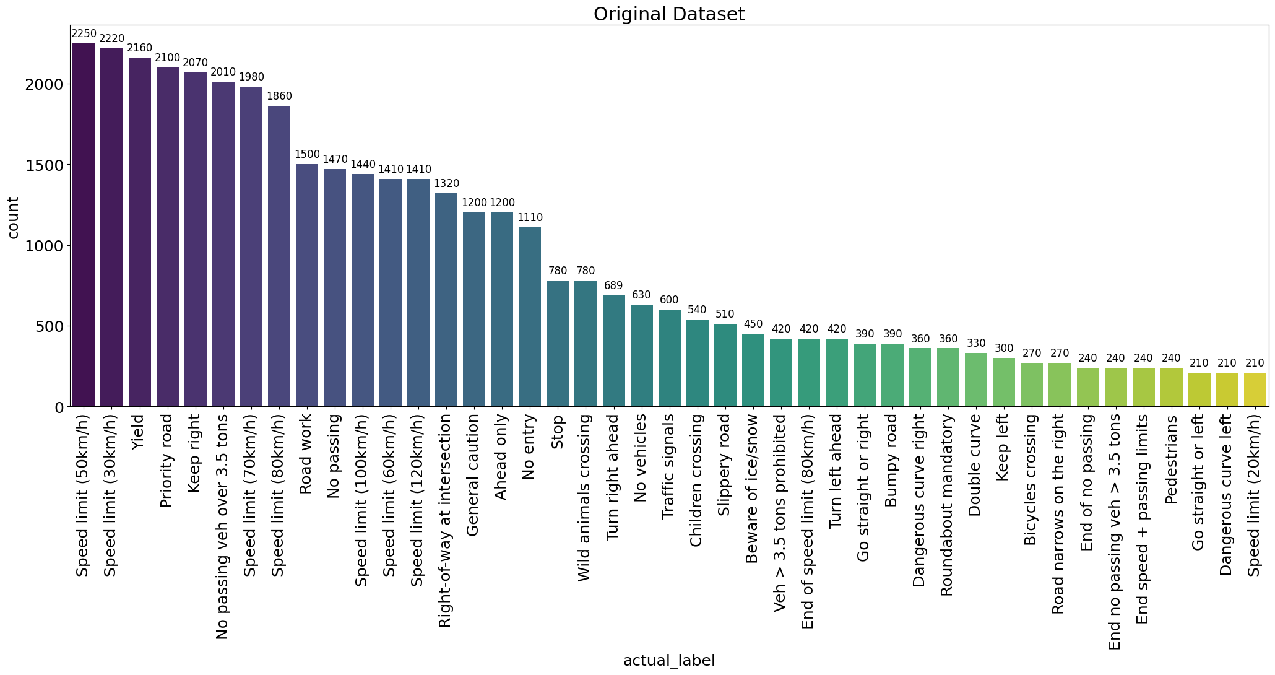
\includegraphics[width=0.95\linewidth]{img/data/evalDist/or.pdf}
        \caption{Class distribution, original.}
    \end{subfigure}
    \begin{subfigure}{0.35\textwidth}
        \centering
        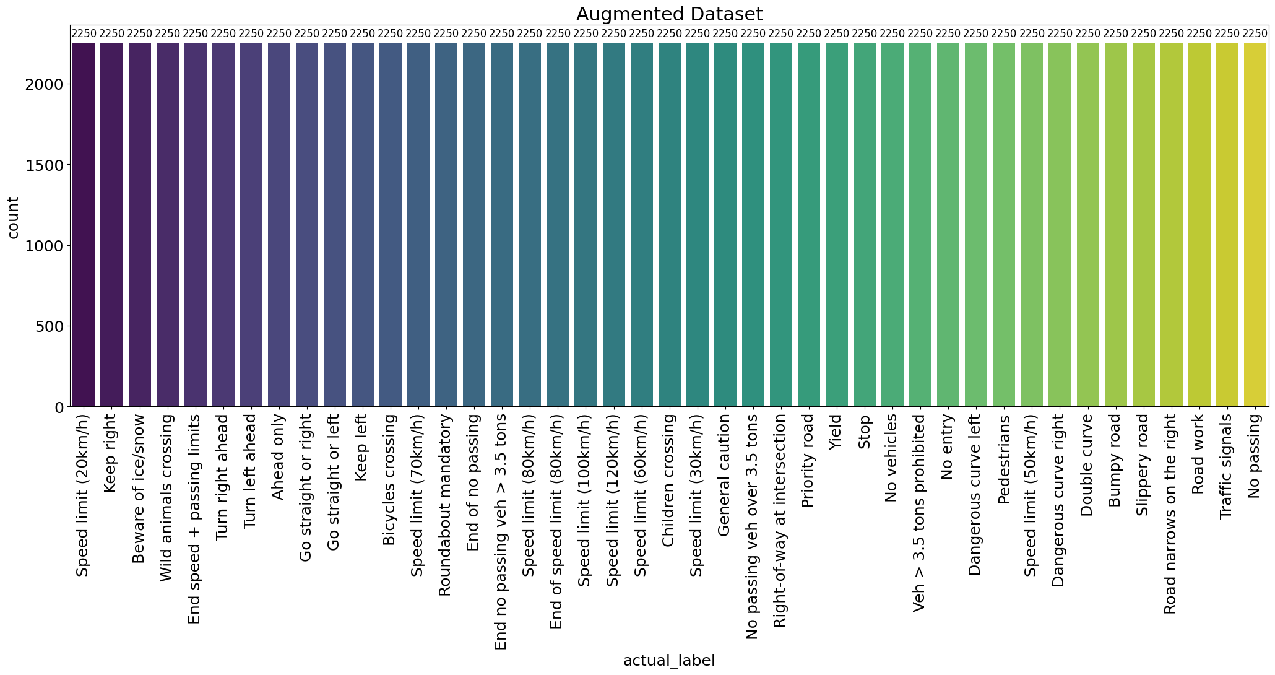
\includegraphics[width=0.95\linewidth]{img/data/evalDist/aug.pdf}
        \caption{Class distribution, augmented.}
    \end{subfigure}
    \begin{subfigure}{0.35\textwidth}
        \centering
        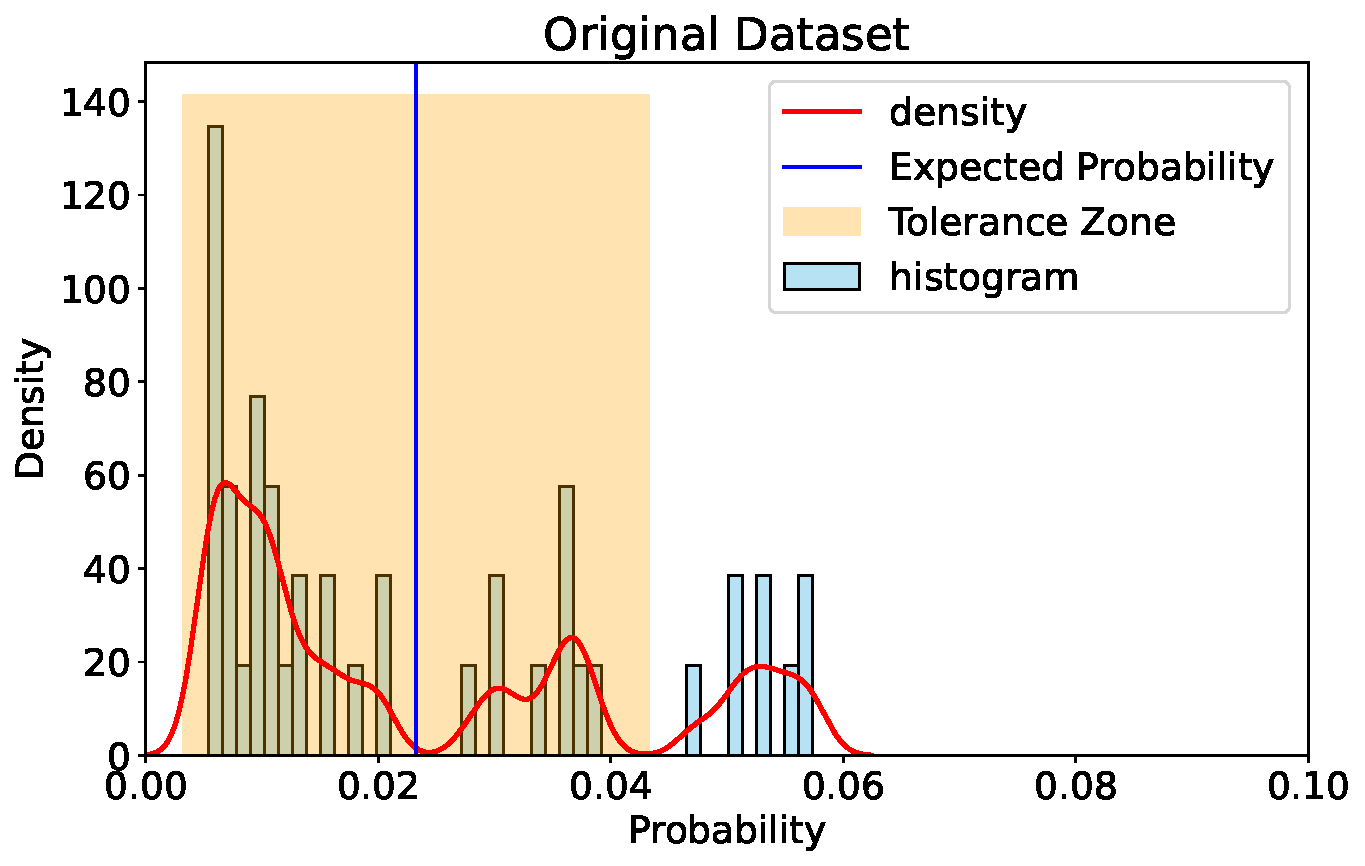
\includegraphics[width=0.95\linewidth]{img/data/evalDist/orp.pdf}
        \caption{Probability distribution, original.}
    \end{subfigure}
    \begin{subfigure}{0.35\textwidth}
        \centering
        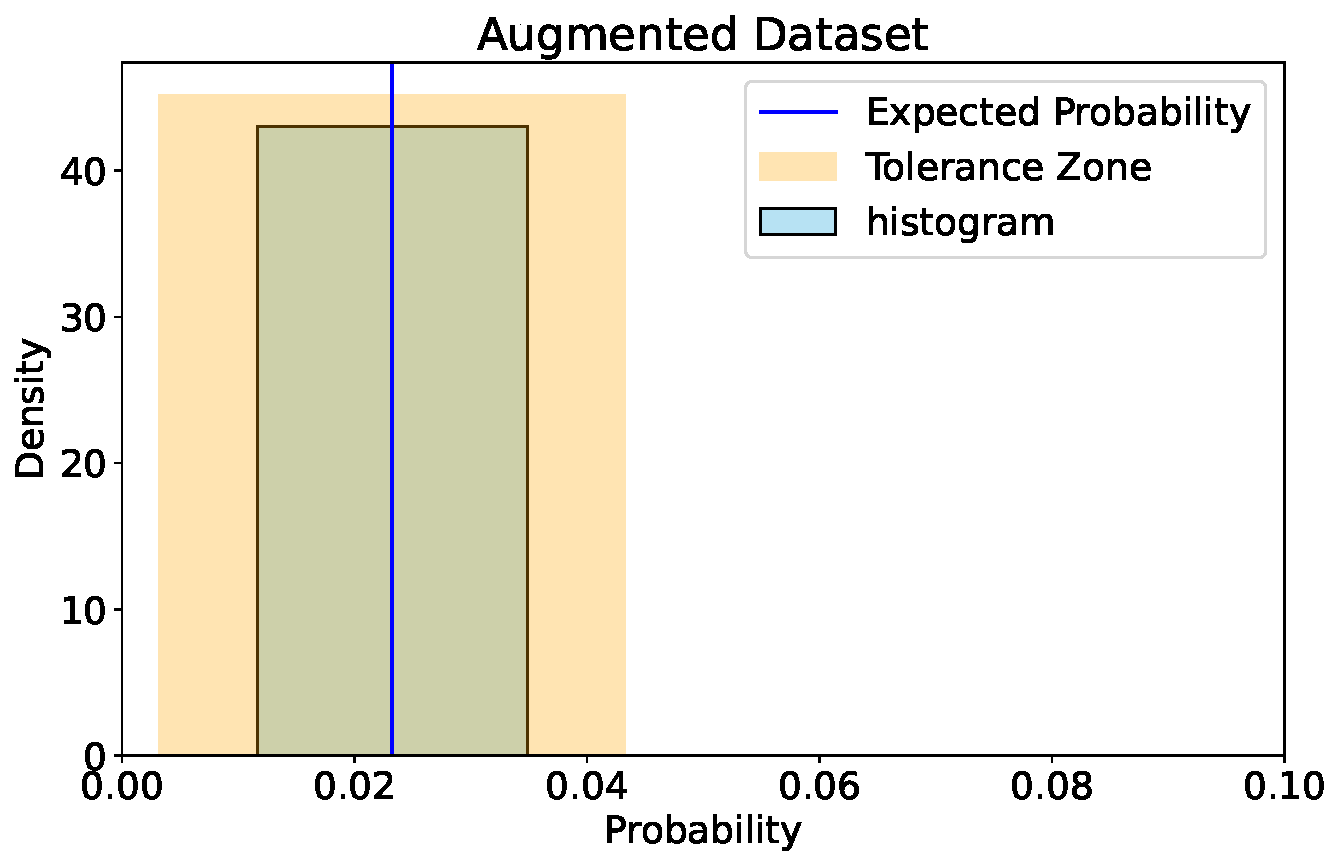
\includegraphics[width=0.95\linewidth]{img/data/evalDist/augp.pdf}
        \caption{Probability distribution, augmented.}
    \end{subfigure}
    \caption{Class distribution and class-probabilities distribution for
      Scenario~1 ($N = 39{,}209$ before and $96{,}750$ after augmentation). Augmentation flattens the class distribution and
      concentrates the probability density at $1/K \approx 0.0233$.}
    \label{fig:gtsrb:distscenario1}
\end{figure}

\begin{table}[!htbp]
\centering
\begin{tabular}{lcc}
\toprule
& \textbf{Original} & \textbf{Augmented} \\
\midrule
Dataset size $N$         & $39{,}209$             & $96{,}750$ \\
Accuracy                 & $95.17\%$              & $95.10\%$ \\
Accuracy on warning signs & $95.19\%$             & $95.40\%$ \\
Accuracy on other signs  & $89.95\%$              & $91.68\%$ \\
Accuracy gap             & $5.24$ pp              & $3.88$ pp \\
GD trust opinion $(b,d,u)$  & $(0.50, 0.11, 0.39)$   & $(0.64, 0.00, 0.36)$ \\
\bottomrule
\end{tabular}
\caption{Scenario~1 (centralized): downstream accuracy and GD trust
  opinion for the original and augmented \ac{GTSRB}.}
\label{tab:gtsrb:acc1}
\end{table}

\paragraph{Scenario~2: collaborative dataset with $M$ contributors.}
We progressively increase the number of imbalanced contributors out of $M$ and observe both the downstream accuracy and the trust opinion produced by each trust source. Downstream accuracy (\cref{fig:gtsrb:accplot}, $M = 100$) shows the expected pattern: warning-sign accuracy collapses from $83\%$ to $0\%$ as the number of imbalanced contributors grows, while accuracy on the other signs degrades gradually (the ``whole test set'' curve nearly coincides with the ``other signs'' curve because warning signs are a small fraction of the test set). The accuracy gap grows accordingly.

The trust opinions (\cref{fig:gtsrb:op}) tell a more nuanced story. The \emph{GD trust source}, applied to the union of all sub-datasets, shows belief decreasing slowly until roughly 60 imbalanced contributors out of 100, after which it drops sharply. This matches the ground truth: the warning-sign classes only leave the tolerance zone once most of their images have been removed. Its uncertainty stays constant at $\approx 0.4$ because the total dataset size $N$ barely changes (only warning-sign images are removed) and \cref{eq:gtsrb:uncertainty} depends only on $N$. The \emph{LE trust source} produces a linear decrease of belief and a symmetric increase of disbelief: each imbalanced contributor adds exactly one unit of negative evidence (\cref{eq:gtsrb:method2-evidence}), so the opinion moves deterministically from $(1, 0, 0.02)$ to $(0, 1, 0.02)$ as the sweep progresses. It is thus more sensitive than the GD trust source to the \emph{number} of problematic contributors, but blind to how much of the global distribution they actually distort, which is the complementarity discussed above.

When the same experiments are repeated with $M = 10$ contributors, the GD trust source shows essentially the same belief/disbelief curves (because $N$ and the global distribution are the same), while the LE trust source exhibits a higher residual uncertainty ($u = 2/12 \approx 0.17$) reflecting the smaller number of evidence sources $r + s = M$ in the \ac{BPQ} formula.

\begin{figure}[!htbp]
    \centering
    \begin{subfigure}{0.48\textwidth}
        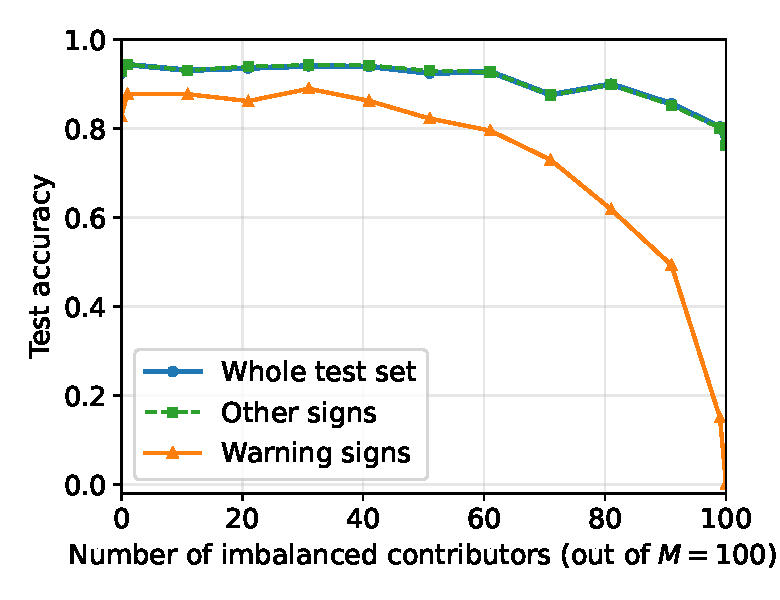
\includegraphics[width=\linewidth]{img/data/res/acc.pdf}
        \caption{Test accuracy.}
    \end{subfigure}
    \hfill
    \begin{subfigure}{0.48\textwidth}
        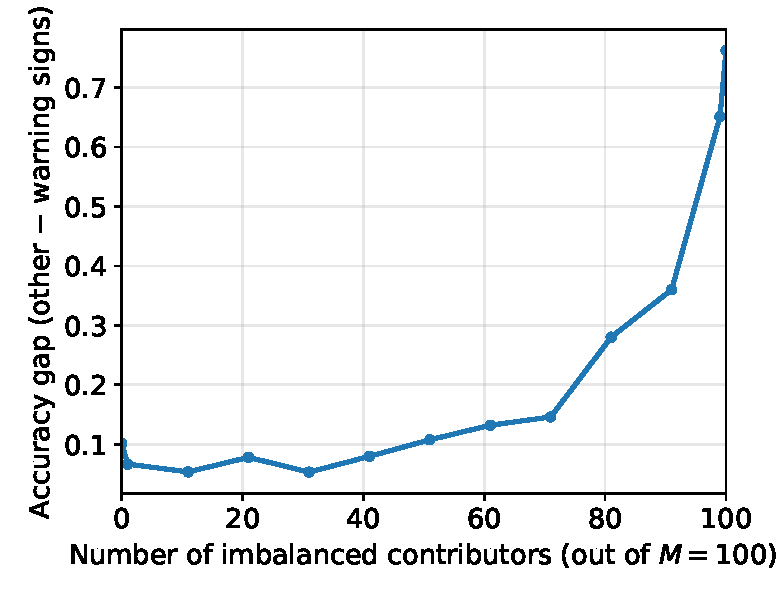
\includegraphics[width=\linewidth]{img/data/res/diff.pdf}
        \caption{Accuracy gap.}
    \end{subfigure}
    \caption{Scenario~2 ($M = 100$): test accuracy on the whole test set, on the warning signs and on the other signs, and the resulting accuracy gap, as a function of the number of imbalanced contributors. The whole-test curve nearly coincides with the other-signs curve because warning signs are a small fraction of the test set.}
    \label{fig:gtsrb:accplot}
\end{figure}

\begin{figure}[!htbp]
    \centering
    \begin{subfigure}{0.35\textwidth}
        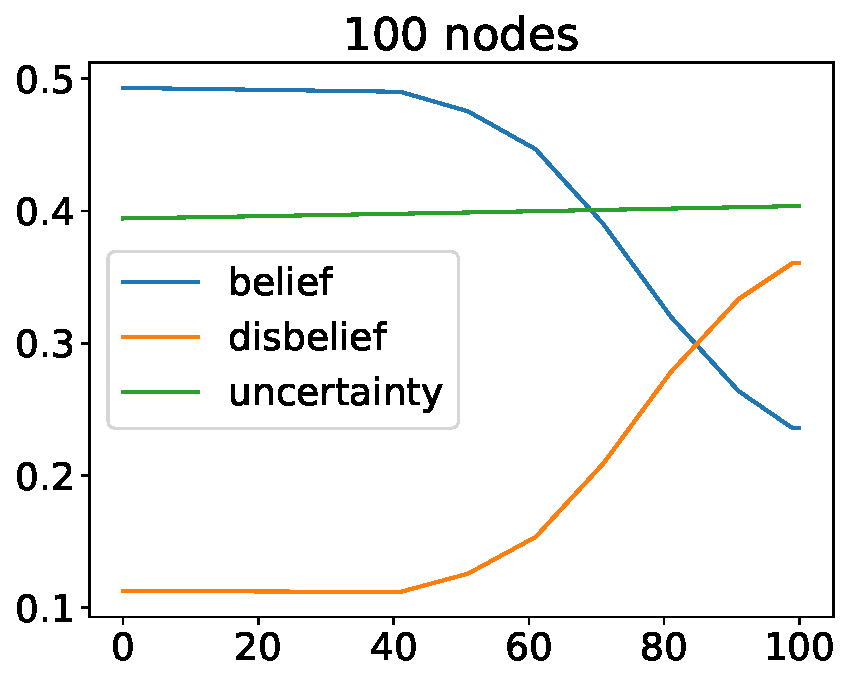
\includegraphics[width=0.95\linewidth]{img/data/res/meth1-100.pdf}
        \caption{GD trust source, $M = 100$.}
    \end{subfigure}
    \begin{subfigure}{0.35\textwidth}
        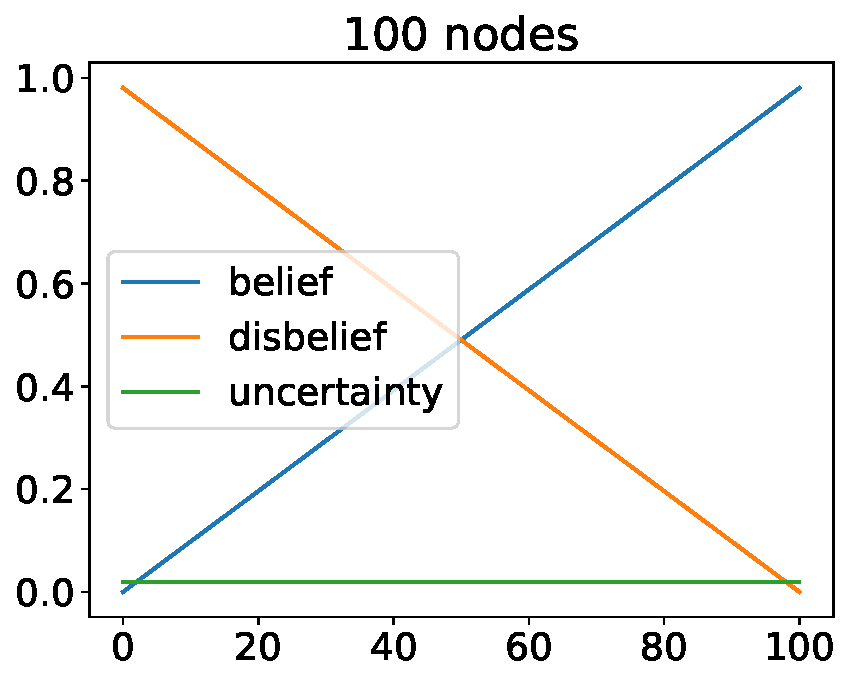
\includegraphics[width=0.95\linewidth]{img/data/res/meth2-100.pdf}
        \caption{LE trust source, $M = 100$.}
    \end{subfigure}
    \begin{subfigure}{0.35\textwidth}
        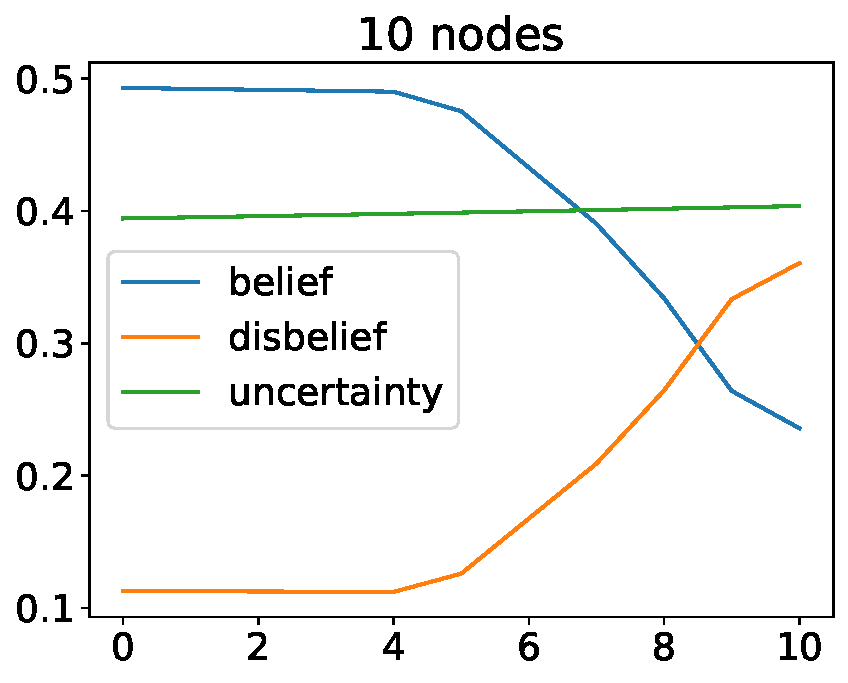
\includegraphics[width=0.95\linewidth]{img/data/res/meth1-10.pdf}
        \caption{GD trust source, $M = 10$.}
    \end{subfigure}
    \begin{subfigure}{0.35\textwidth}
        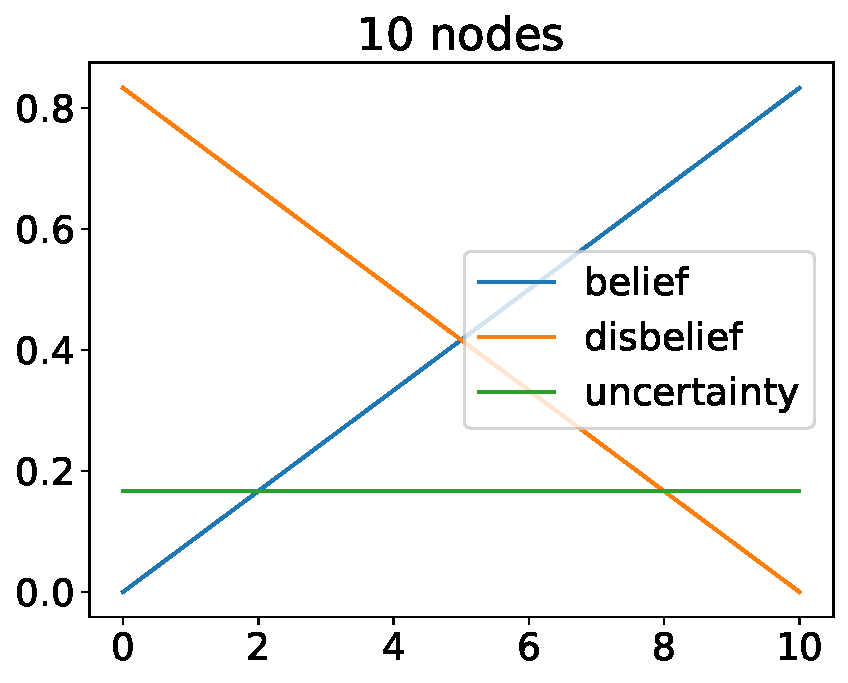
\includegraphics[width=0.95\linewidth]{img/data/res/meth2-10.pdf}
        \caption{LE trust source, $M = 10$.}
    \end{subfigure}
    \caption{Trust opinions $(b, d, u)$ produced by the GD and LE trust sources for
      $M = 10$ and $M = 100$ contributors, as a function of the number of imbalanced
      contributors ($x$-axis). The GD uncertainty is constant because the total
      dataset size $N$ is unchanged; the LE opinion moves linearly because each imbalanced contributor adds one unit of negative evidence.}
    \label{fig:gtsrb:op}
\end{figure}

\paragraph{Sensitivity to the tolerance $\eta$.}
The tolerance $\eta$ controls how strictly the GD trust source interprets balance. Too small a value penalizes minor imbalances; too large a value lets substantial imbalances pass undetected. \Cref{fig:gtsrb:eta_effect} shows belief, disbelief and uncertainty as functions of $\eta$ on the original \ac{GTSRB}. Belief rises and stabilizes as $\eta$ grows, disbelief drops correspondingly, and uncertainty stays constant as expected from \ac{CUQ}. The shaded region ($0.0185 \leq \eta \leq 0.0235$) marks a \emph{stability zone} in which the trust opinion is insensitive to small changes of $\eta$. We pick $\eta = 0.02$ for all reported experiments because it lies in the middle of this zone; this is an instance of the sensitivity-analysis recommendation of \cref{sec:dataset-trust:framework:hyperparameters}.

\begin{figure}[!htbp]
  \centering
  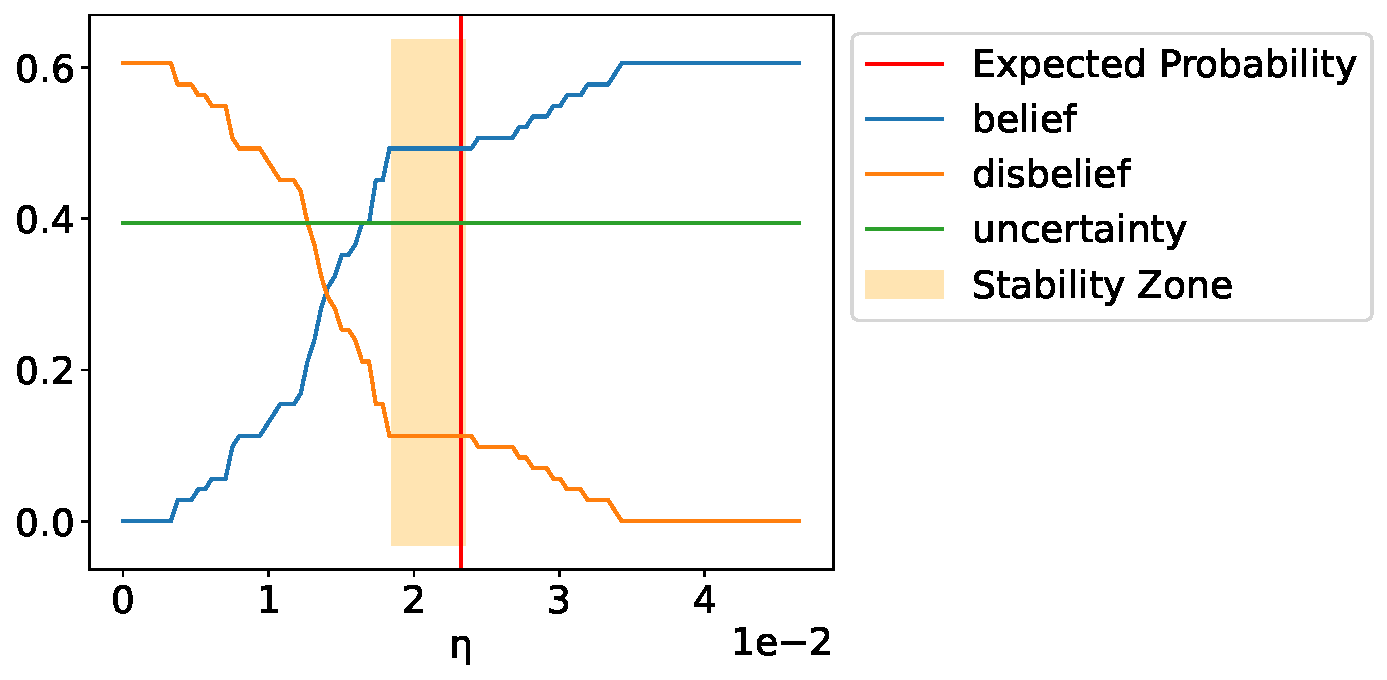
\includegraphics[width=0.7\linewidth]{img/data/eta.pdf}
  \caption{Effect of $\eta$ on the belief, disbelief and uncertainty of the GD trust source on the original \ac{GTSRB}. The red vertical line marks
    the expected probability $1/K \approx 0.02326$. The shaded region
    ($0.0185 \leq \eta \leq 0.0235$) is the stability zone in which the
    opinion is insensitive to small changes of $\eta$. Uncertainty is
    constant because the GD trust source fixes it externally via \cref{eq:gtsrb:uncertainty}.}
  \label{fig:gtsrb:eta_effect}
\end{figure}

\subsection{What this application showed}
\label{sec:gtrsb_summary}

Returning to the research question: for the proposition ``$\dataset$ is not biased with respect to class balance'', both trust sources produced opinions that track the known imbalance and its downstream effect. In Scenario~1 the GD opinion separated the original dataset (eight classes outside the tolerance zone, $d = 0.11$) from the balanced one ($d = 0$), in line with the reduction of the accuracy gap. In Scenario~2 both opinions moved toward disbelief as contributors became imbalanced and the warning-sign accuracy collapsed, but along different curves that reflect what each trust source can observe.

The two trust sources answer the same proposition by different routes and have complementary strengths. The GD trust source requires the global class-probabilities distribution and is the natural choice when the dataset is centralized and observable. The LE trust source only requires one scalar per contributor and is therefore the natural choice in collaborative or federated settings where class counts cannot be shared, at the price of the complementarity blind spot discussed in \cref{sec:dataset-trust:applications:gtsrb:method2}. They also illustrate two different quantification schemes: the GD trust source fixes uncertainty externally via sample complexity, which is appropriate when the dataset size is the bottleneck of the assessment's confidence; the LE trust source lets uncertainty shrink as more contributors provide evidence, which is appropriate when the unit of evidence is one local assessment per contributor. The same proposition can therefore be assessed under \ac{CUQ} or \ac{BPQ} depending on whether ``more evidence'' means ``more data'' or ``more contributors''.

Two caveats apply. Class imbalance is not always a defect: in some applications it faithfully reflects the deployment-time class frequencies, and forcing balance would degrade rather than improve the model. A natural extension of the GD trust source replaces the uniform expected probability $1/K$ with a deployment-derived target distribution, preserving the rest of the procedure. And the sample-complexity bound used to set $U$ is conservative, so the absolute level of uncertainty ($\approx 0.4$) should be read as a relative scale across datasets rather than as a calibrated probability.

\FloatBarrier

% ==============================================================
\section{Annotation Stage, Entry Level: Labeling accuracy on \\CIFAR-10H}
\label{sec:dataset-trust:applications:cifar10h}

\begin{mdframed}[backgroundcolor=blue!4, linewidth=0pt]
\textbf{Position in the design space.}

$\propP$ = accuracy (of labels);\quad
$\propS = \{\textsc{annotation}\}$;\quad
$\propG$ = entry;\

\textbf{Quantification:} \ac{BPQ} (evaluated), \ac{EWQ} (discussed).\quad

\textbf{Purpose:} evaluation.\quad \textbf{Published in:}~\cite{trust-aidatatrust}.
\end{mdframed}

\paragraph{Purpose and research question.}
The third application evaluates the framework at the \emph{entry} granularity, where each individual label is a trust proposition of its own. It was chosen because labeling accuracy is the dataset property with the most direct effect on a supervised model and because CIFAR-10H offers something rare: for every image, about fifty independent human labels, so that the disagreement between annotators, which is the evidence the framework uses, is directly observable and can be manipulated. The research question is: \emph{do per-entry opinions derived from annotator agreement identify genuinely ambiguous items, and does their uncertainty respond correctly to the amount of annotation available for each item?} The application also shows how the same construction extends to the annotators themselves, which connects the dataset assessment to the trust-discounting operator of \cref{chap:rw}.

\paragraph{Dataset and annotation scenario.}
CIFAR-10H~\cite{peterson2019human} re-annotates the $10{,}000$ images of the CIFAR-10 test set~\cite{krizhevsky2009learningcifar} (ten object classes such as \emph{airplane}, \emph{cat}, \emph{truck}). Each image was shown to about $51$ crowdworkers recruited on Amazon Mechanical Turk ($2{,}571$ workers in total, $511{,}400$ labels), each of whom chose one of the ten classes; workers labeled 200 images each, with attention checks. The scenario is thus the standard one of crowdsourced labeling: several independent, non-expert annotators label the same item, and the dataset curator has to decide on one label per item. In CIFAR-10H, as in most crowdsourcing pipelines, that decision is taken by \emph{majority vote} over the annotators; the majority label is the one we assess. The original CIFAR-10 label is also available and agrees with the majority label for the vast majority of images, which is why the dataset is a good testbed: disagreement among annotators concentrates on genuinely ambiguous images (e.g., a cat that looks like a dog) rather than on random noise~\cite{peterson2019human}.

\paragraph{Trust proposition.}
For each image $x$, the proposition is \emph{``the decision label $y^\prime$ for $x$ is accurate,''} where $y^\prime$ is the majority label. Each image is assessed independently, producing a per-entry opinion $\omega_{x} = (b_{x}, d_{x}, u_{x})$. The set of per-entry opinions can be lifted into a dataset-level opinion on labeling accuracy with the cross-granularity mechanisms of \cref{sec:dataset-trust:formal:granularity}.

\subsection{Trust source: divergence to the decision label}
\label{sec:dataset-trust:applications:cifar10h:source}

The trust source operates at the level of individual annotators. For each annotator $j$ of instance $x$, we compute a divergence score $d_j(x)$ that measures how far the annotator's response is from the decision label $y^\prime$. For categorical annotations, $d_j(x) = 0$ when the annotator agrees with $y^\prime$ and $d_j(x) = 1$ otherwise; for probabilistic annotations, \ac{KL} divergence or cross-entropy between the annotator's distribution and $y^\prime$ is a natural choice; for free-text annotations, semantic distance (e.g., cosine distance between embeddings) plays the same role.

A divergence threshold $\delta$ separates evidence supporting the proposition from evidence against it:
\begin{equation}
r_x = \big|\{j : d_j(x) \leq \delta \}\big|,
\qquad
s_x = \big|\{j : d_j(x) > \delta \}\big|.
\label{eq:cifar10h:evidence}
\end{equation}

The threshold $\delta$ can be set in several ways depending on the annotation modality and on what reference information is available.

\noindent \emph{By edge-case construction}, $\delta$ is set to the divergence that an \emph{edge-acceptable} annotation would produce relative to the decision label: that is, an annotation that is the most distant response still considered acceptable for the given label, by analogy with the edge-acceptable distribution used to set the threshold of the LE trust source in the \ac{GTSRB} application (\cref{sec:dataset-trust:applications:gtsrb:method2}).

\noindent \emph{By domain policy}, $\delta$ is fixed by external requirements, e.g., $\delta = 0$ for categorical labels (strict agreement) and $\delta = 0.1$ for soft labels.

\cref{alg:cifar10h:opinions} summarizes the construction of per-entry opinions.

\begin{algorithm}[!htbp]
\caption{Per-entry opinion construction from annotations}
\label{alg:cifar10h:opinions}
\label{alg:opinions}
\begin{algorithmic}[1]
\Require Annotations $\{y_j(x)\}$ or $\{p_j(x)\}$, decision label $y^\prime$,
threshold $\delta$, prior weight $W$
\For{each instance $x$}
  \State $r_x \leftarrow |\{j : \mathrm{divergence}(y_j(x), y^\prime) \leq \delta \}|$
  \State $s_x \leftarrow |\{j : \mathrm{divergence}(y_j(x), y^\prime) > \delta \}|$
  \State $b_x \leftarrow r_x / (W + r_x + s_x)$
  \State $d_x \leftarrow s_x / (W + r_x + s_x)$
  \State $u_x \leftarrow W / (W + r_x + s_x)$
  \State Output opinion $\omega_x = (b_x, d_x, u_x, a)$
\EndFor
\end{algorithmic}
\end{algorithm}

\paragraph{Quantification schemes: \ac{BPQ} and \ac{EWQ}.}
The trust source produces evidence counts $(r_x, s_x)$ that grow with the number of annotators $n = r_x + s_x$ of instance $x$. This makes two quantification schemes natural. \ac{BPQ}, with prior weight $W$, gives uncertainty $u_x = W / (W + n)$: residual uncertainty decreases as more annotators contribute, which is the desired behavior when annotation volume varies across instances. \ac{EWQ} additionally assumes that each annotation comes with its own uncertainty weight. It is relevant when annotators self-report a confidence score alongside their label, or when external metadata provides a per-annotation reliability proxy (e.g., annotation duration). Where \ac{BPQ} lets the \emph{amount} of evidence drive uncertainty, \ac{EWQ} lets the \emph{quality} of each piece of evidence drive it. CIFAR-10H records neither confidence nor duration, so only \ac{BPQ} is evaluated below.

\paragraph{Worked example.}
Consider an instance $x$ annotated by $50$ crowdworkers, of whom $46$ agree with the decision label and $4$ disagree, with $\delta = 0$ and $W = 2$. \cref{eq:cifar10h:evidence} gives $r_x = 46$, $s_x = 4$, and \ac{BPQ} gives:
\begin{equation}
b_x = \tfrac{46}{52} \approx 0.885,\quad
d_x = \tfrac{4}{52} \approx 0.077,\quad
u_x = \tfrac{2}{52} \approx 0.038.
\end{equation}
The opinion captures three qualitatively different signals simultaneously: high belief reflecting strong agreement, residual disbelief reflecting genuine disagreement among annotators, and low uncertainty reflecting that the evidence base is large.

\paragraph{Annotator-level extension.}
The same construction applies to a different entity: the annotators themselves. For annotator $j$, partitioning $j$'s responses across all the items $j$ labeled into agreements and disagreements with the corresponding decision labels yields evidence counts $(r_j, s_j)$ for the proposition \emph{``annotator $j$ is reliable''}. Applying \ac{BPQ} to $(r_j, s_j)$ produces a per-annotator opinion $\omega_j$ on the same $(b, d, u)$ scale as the per-entry opinions.

This construction implicitly assumes that more than half of the annotators are honest and competent: the decision label $y^\prime$ is taken as the reference against which each annotator is judged, so the resulting reliability opinion is only meaningful if the procedure that produced $y^\prime$ is itself reliable. If $y^\prime$ is set by majority vote, the assumption is that the majority of annotators is correct on most items. In settings where this fails (e.g., adversarial annotators colluding to flip the majority on targeted items), $\omega_j$ would conflate genuine reliability with mere conformity to a corrupted reference.

\paragraph{Connection to trust discounting.}
The per-annotator opinion is exactly the \emph{referral} trust opinion expected by the trust-discounting operator of \cref{subsec:TD_operators}. In the terminology of \cref{def:two_edge_discounting}, the curator $A$ holds a referral opinion $\omega^A_j = \omega_j$ about annotator $j$, and annotator $j$ holds a functional opinion about the proposition ``$y^\prime$ is accurate for $x$'': a categorical vote is the dogmatic opinion $\omega^j_x = (1, 0, 0)$ if $j$ agrees with $y^\prime$ and $(0, 1, 0)$ otherwise. Two-edge discounting gives the curator's opinion via $j$,
\[
\omega^{[A;j]}_x = \omega^A_j \otimes_{TE} \omega^j_x =
\begin{cases}
(P_j,\ 0,\ 1 - P_j) & \text{if } j \text{ agrees with } y^\prime,\\
(0,\ P_j,\ 1 - P_j) & \text{otherwise},
\end{cases}
\]
where $P_j = b_j + a\,u_j$ is the projected probability of $\omega_j$, and the per-entry opinion is the cumulative fusion $\bigoplus_j \omega^{[A;j]}_x$ over the annotators of $x$. In evidence terms, this replaces the plain counts of \cref{eq:cifar10h:evidence} by counts weighted by the annotators' reliability, $r_x = \sum_{j \text{ agrees}} P_j$ and $s_x = \sum_{j \text{ disagrees}} P_j$: a fully reliable annotator contributes one unit of evidence, an unreliable one contributes less, and the difference is turned into uncertainty rather than discarded. The labeling-accuracy assessment thus becomes a two-level instantiation of the General Methodology: the proposition ``$y^\prime$ is accurate'' is supported by referral evidence from annotators whose own reliability is an assessable proposition.

\subsection{Experimental evaluation}
\label{sec:dataset-trust:applications:cifar10h:eval}

We evaluate the trust source on the full CIFAR-10H ($10{,}000$ images, about $51$ annotations each). The decision label $y^\prime$ of each image is its majority label, the divergence threshold is $\delta = 0$ (strict agreement) and the prior weight is $W = 2$.

\Cref{fig:cifar10h:masses} compares the empirical distribution of $(b_x, d_x, u_x)$ over the $10{,}000$ images in two settings: the full dataset, and a \emph{cropped} variant in which each image is reduced to $10$ annotations by removing responses from the majority label only, so that the cropped set retains all minority annotations while reducing the dominant agreement signal. This manipulation is designed to answer the second half of the research question: it changes the amount of evidence per item without changing which items are ambiguous.

Two effects are visible. First, on the full dataset belief concentrates near $1$ and uncertainty near $0$: with about $50$ annotators per image, $u_x = W / (W + 50) \approx 0.04$ regardless of the agreement ratio. This high apparent confidence is partly an artifact of evidence saturation rather than a genuine signal of label quality, and it is the correct behavior of \ac{BPQ}: fifty independent votes \emph{are} a lot of evidence about a majority label. The items that matter are the outliers of the belief box plot, i.e., the images on which a sizeable minority of annotators disagreed; these are, by construction, the images on which CIFAR-10H's annotators disagree, which~\cite{peterson2019human} report to be visually ambiguous rather than randomly mislabeled. Second, the cropped setting redistributes mass across the three components: disbelief becomes visible for items with annotator disagreement, and uncertainty rises mechanically to $u_x = W / (W + 10) \approx 0.17$. The opinions are now informative about the actual difficulty of each item, with controversial instances showing simultaneously low belief and high disbelief, while unanimous ones keep $d_x = 0$.

\begin{figure}[!htbp]
    \centering
    \begin{subfigure}[b]{0.49\textwidth}
        \centering
        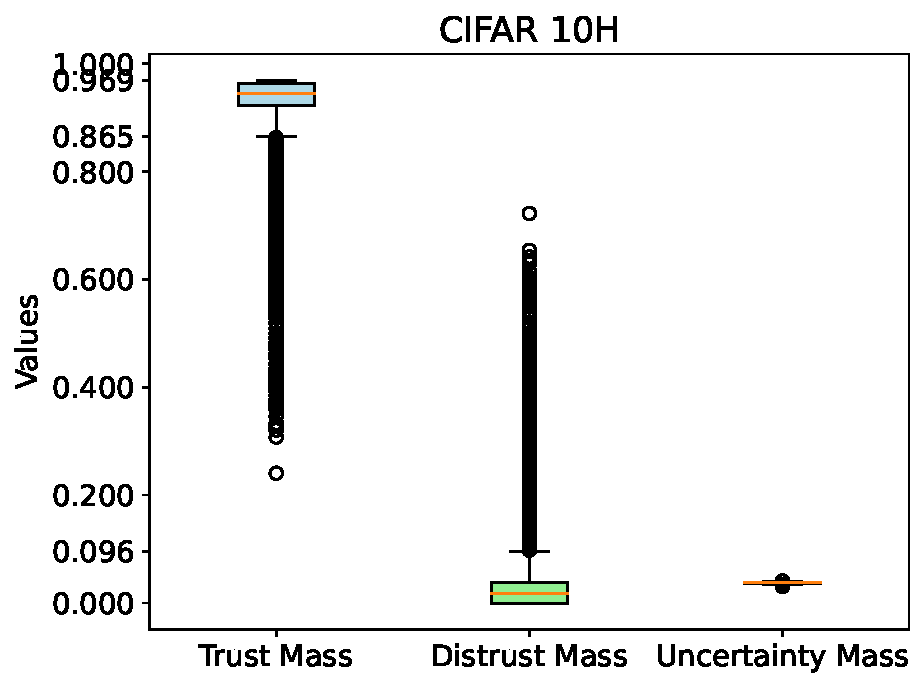
\includegraphics[width=\textwidth]{img/data/CIFAR_10H.pdf}
        \caption{Full CIFAR-10H ($\approx 50$ annotators per item).}
    \end{subfigure}
    \hfill
    \begin{subfigure}[b]{0.49\textwidth}
        \centering
        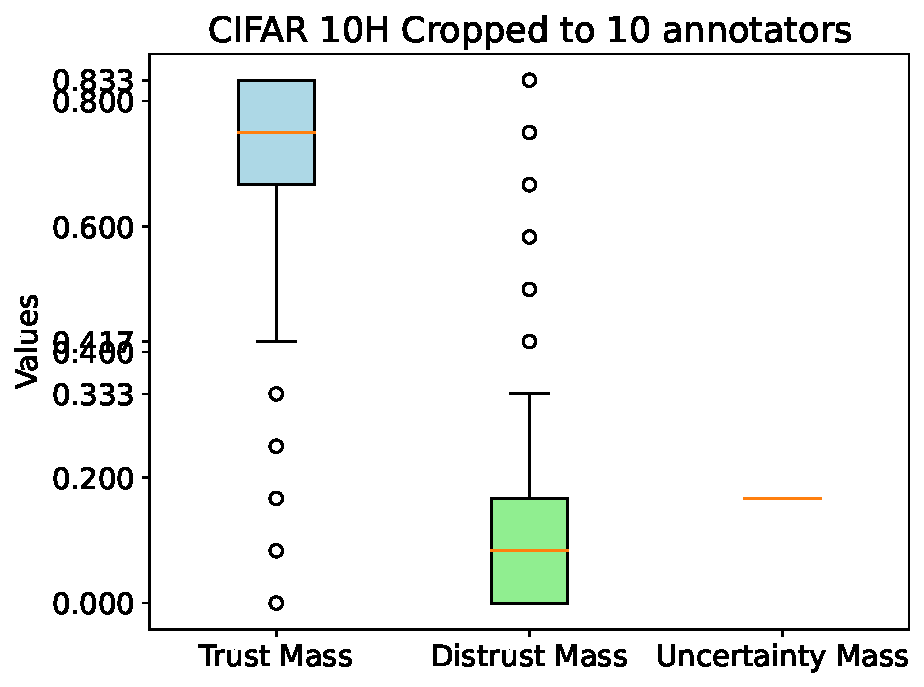
\includegraphics[width=\textwidth]{img/data/CIFAR_10H_Cropped.pdf}
        \caption{Cropped to $10$ annotators per item by removing majority-label responses.}
    \end{subfigure}
    \caption{Box plots of belief, disbelief and uncertainty over the $10{,}000$ images of
      CIFAR-10H. The full dataset shows high belief and low
      uncertainty driven primarily by evidence saturation. The cropped
      setting redistributes mass across the three components and surfaces
      genuine annotator disagreement.}
    \label{fig:cifar10h:masses}
\end{figure}

\subsection{What this application showed}
\label{sec:dataset-trust:applications:cifar10h:discussion}

Returning to the research question: the per-entry opinions single out the ambiguous images through their disbelief mass, and their uncertainty responds to the amount of annotation exactly as \ac{BPQ} prescribes ($0.04$ with $50$ annotators, $0.17$ with $10$), independently of the agreement ratio. This separation is what a scalar agreement rate cannot provide: an image with $9$ agreeing annotators out of $10$ and an image with $45$ out of $50$ have the same agreement rate but different opinions, $(0.75, 0.08, 0.17)$ versus $(0.87, 0.10, 0.04)$, the second being held with more confidence.

Per-annotator opinions $\omega_j$ can in turn be used to filter unreliable contributors, to reweight their evidence through the discounting construction above, or to drive targeted re-annotation. This application covers the annotation stage at entry granularity, exercises \ac{BPQ}, discusses where \ac{EWQ} would apply, illustrates the cross-granularity composition of \cref{sec:dataset-trust:formal:granularity}, and connects to the trust-discounting operator via the annotator-level extension. Together with the \ac{GTSRB} application, it covers the two canonical routes to a dataset-level assessment: direct global evidence (\ac{GTSRB}) and lifted entry-level evidence (CIFAR-10H).

\noindent \cref{tab:dataset-trust:applications-summary} summarizes the position of the three applications in the design space.

\begin{table}[!htbp]
  \centering
  \small
  \renewcommand{\arraystretch}{1.2}
  \begin{tabular}{@{}llll@{}}
    \toprule
     & \textbf{COMPAS} & \textbf{GTSRB} & \textbf{CIFAR-10H} \\
    \midrule
    Property $\propP$        & overall trustworthiness & representativeness & labeling accuracy \\
    Stage(s) $\propS$        & all four                & sampling           & annotation \\
    Granularity $\propG$     & dataset                 & dataset            & entry \\
    Quantification           & \acs{BPQ}               & \acs{CUQ}, \acs{BPQ} & \acs{BPQ} (\acs{EWQ} discussed) \\
    Purpose                  & illustration            & evaluation         & evaluation \\
    \midrule
    Dataset source           & ProPublica~\cite{angwin2016machine} & \cite{stallkamp2012man} & \cite{peterson2019human} \\
    Published in             & this dissertation       & \cite{10.1007/978-3-032-19096-3_17} & \cite{trust-aidatatrust} \\
    \bottomrule
  \end{tabular}
  \caption{Position of each application in the three-axis design space of
    \cref{sec:dataset-trust:framework:design-space}, the quantification scheme it exercises, its purpose, the origin of the dataset and the publication in which it first appeared.}
  \label{tab:dataset-trust:applications-summary}
\end{table}

\FloatBarrier

% ==============================================================
\section{Summary \& Conclusions} \label{sec:dataset-trust:summary}

This chapter introduced a framework for assessing the trustworthiness of \ac{AI} training datasets by specializing the general methodology of \cref{chap:Trust_method}. Its central claim is that dataset trustworthiness should be treated not as a single score, but as a structured assessment defined by three dimensions: the property assessed, the lifecycle stage from which evidence is collected, and the granularity at which it applies.

The framework rests on three artifacts. First, the lifecycle decomposition (sampling, collection, annotation, processing) and the trust-source catalogue fix the \emph{structure} of an assessment: a two-level trust expression whose leaves are trust sources selected by property, stage and granularity. Second, the quantification procedure turns the value of a trust source into evidence (through threshold-based normalization and an evidence strength) and evidence into an opinion (through \ac{BPQ}, \ac{EWQ} or \ac{CUQ}), with explicit, reportable hyperparameters. Third, the cross-granularity composition mechanisms (opinion composition and evidence lifting) let evidence collected at feature or entry level support entry- or dataset-level propositions.

Three applications instantiated the framework. \ac{COMPAS} illustrated multi-stage composition on a real tabular dataset and showed that the stage-level opinions distinguish a stage weakened by negative evidence from a stage that merely lacks evidence. \ac{GTSRB} evaluated two trust sources for class balance against a known, controllable imbalance and its effect on a \ac{CNN}, in centralized and federated settings, and showed that the same proposition can be quantified under \ac{CUQ} or \ac{BPQ} depending on what is observable. CIFAR-10H evaluated entry-level opinions against directly observable annotator disagreement and showed that belief, disbelief and uncertainty separate ambiguity from lack of annotation.

The framework provides richer decision support than scalar metrics. An opinion $(b, d, u)$ distinguishes supporting evidence, contradicting evidence, and uncertainty. This enables auditors to differentiate between lack of evidence and conflicting evidence, two situations requiring different actions, making the framework a diagnostic tool rather than a pass/fail measure.

\paragraph{Limitations.}
Three limitations remain. First, the trust-source catalogue is not exhaustive: it lists the trust sources considered in this thesis, and applying the framework to a concrete system will typically require defining additional ones, which the catalogue accommodates as long as they are placed at a stage, a risk category and a granularity. Second, the hyperparameters ($\tau_m$, $A_m$, $L_m$, $K_m$, $W$, $U$) must be set by the analyst. \cref{sec:dataset-trust:framework:hyperparameters} gives guidance (requirements or expert elicitation for thresholds, with sensitivity analysis as a safeguard; uniform $K_m$ unless source authority differs; $W = 2$ unless evidence is noisy), and the $\eta$ sensitivity analysis of \cref{sec:dataset-trust:applications:gtsrb:eval} shows that partial calibration is feasible, but the assessment remains only as meaningful as these choices, which is why they must be reported with it. Third, the lifecycle stages enter the conjunction of \cref{eq:dataset-trust:lifecycle-decomposition} with equal weight, whereas a task may warrant weighting them differently: for a fairness audit of a hiring dataset the annotation stage (who assigned the outcome labels) dominates, whereas for a sensor-fusion dataset the collection stage (calibration and drift) does. Such weighting can be expressed within \ac{SL} by discounting the stage-level opinions with a task-dependent referral opinion before the conjunction, which is left to future work.

\paragraph{Relation to the Trust Propagation Module.}
The framework outputs trust opinions at dataset, entry or feature granularity. These are the inputs of the Trust Propagation Module of \ac{PaTAS}, presented and evaluated in \cref{chap:patas}, which operates on per-feature trust opinions. A coarser-grained (dataset- or entry-level) opinion can be replicated at the feature level, enabling propagation through the model parameters during training. At inference time, the same trust sources applied to the features of an individual input yield per-feature opinions, which are propagated through the network to produce an output trust opinion. Replicating a dataset-level opinion onto every input, however, gives every input the same trust regardless of its individual quality, which limits the value of per-instance trust evaluation at inference. Input-level assessment should therefore \emph{add} entry- or feature-level trust sources computed on the individual input to the dataset-level opinion, rather than replace one by the other: the dataset-level opinion captures what the model was trained on, the input-level opinion what it is being asked about, and both enter the propagation.

Finally, while the training-dataset assessment and the inference-time input assessment may share the same trust property, they do not need to rely on the same trust sources. The analyst is free to use different trust sources for the two, as long as both address the same underlying proposition. For instance, dataset-level accuracy may be supported by sensor-consistency scores computed across the training set, while input-level accuracy at inference time may be supported by an out-of-range check or a per-sensor confidence score applied to the individual input.
